% Learn Latex: https://www.overleaf.com/learn/latex/Learn_LaTeX_in_30_minutes
% using empty line for new paragraph instead of \par

\documentclass[12pt]{article}
\usepackage[utf8]{inputenc}
\usepackage[english]{babel}
\usepackage{indentfirst}
\usepackage{graphicx}
\usepackage{caption}
\usepackage{float}
\usepackage[margin=1.2in]{geometry} % margins
\usepackage{multicol}
\usepackage{wrapfig}
\usepackage{amsmath}
\usepackage{amssymb}
\usepackage[colorlinks=true, linkcolor=blue, urlcolor=cyan]{hyperref}

\graphicspath{{./Figures/}}
\setlength{\parskip}{1em} % paragraph spacing
\renewcommand{\baselinestretch}{1.5} % line spacing
\addto\captionsenglish{\renewcommand{\contentsname}{Units}} % Change TOC title

% custom commands
\newcommand{\fline}{\par\noindent\rule{\textwidth}{0.1pt}} % horizontal line (wide)

\title{\textbf{AP Calculus BC:\\Notes, Formulas,  Equations,\\and Examples}}
\author{Bryan Deng}
\date{Start date: March 2, 2021\\Completed: May 6, 2021}

\begin{document}
\maketitle
\vfill
\begin{center}
    \textit{Sections based off of College Board units.\\
        Formatting may not be the best, this is just a study tool. (Still a work in progress.)}
\end{center}
\newpage

\tableofcontents
\fline
\newpage

\addcontentsline{toc}{section}{Introduction}
\section*{Introduction}
\indent The percentages beside the section titles are how much of the AP Calculus BC exam score will be of that topic. (Based off of College Board website.)

\noindent \textbf{Resources:}
\begin{itemize}
    \item \href{https://apstudents.collegeboard.org/courses/ap-calculus-bc}{College Board Website}
    \item \href{https://www.khanacademy.org/math/ap-calculus-bc}{Khan Academy}
    \item \href{https://www.math24.net/topics-calculus}{Math 24 (Quick explanations of topics)}
    \item \href{https://www.math.ucdavis.edu/~kouba/CalcOneDIRECTORY/}{Practice Questions + Solutions}
    \item \href{https://www.chelmsford.k12.ma.us/site/handlers/filedownload.ashx?moduleinstanceid=2496&dataid=7289&FileName=AP%20Calculus%20BC%20Syllabus.pdf}{BC Exam Syllabus (Not the most organized but good enough)}
\end{itemize}

\section{Limits and Continuity (4\% - 7\%)}
\fline

The limit is when a given value approaches, or gets \textit{really close} (infinitely) to another value. The standard notation for a limit:
\[ \lim_{x \to c} f(x) \]
represents when $x$ can approach $c$ from either the left ($-$) or the right ($+$). By adding a sign superscript to the $c$, it means the $x$ can only approach from that direction:
\[ \lim_{x \to c^+} f(x) \]
\begin{center}
    \textit{Right hand limit}, $x$ approaches $c$ from values greater than $c$.
\end{center}
\[ \lim_{x \to c^-} f(x) \]
\begin{center}
    \textit{Left hand limit}, $x$ approaches $c$ from values greater than $c$.
\end{center}

\subsection{Limits to Infinity}

If a degree (biggest exponent) of a polynomial is greater than or equal to $1$, its limit as $x$ approaches $\pm\infty$ will also be $\pm\infty$. This depends on the sign of the leading coefficient and the degree of the polynomial.

\noindent Example:
\begin{align*}
                         & f(x) = 3x^3 - 7x^2 + 2 \\
    \lim_{x \to \infty}  & f(x) = \infty          \\
    \lim_{x \to -\infty} & f(x) = -\infty
\end{align*}

The degree of $f(x)$ is $3$, and the leading coefficient it positive. The graph goes down to up from left to right.

With Fractions, just find whether the highest degree is in the numerator or the denominator. Numerator means $\infty$, denominator means $0$.

\subsection{Asymptotes}
Sometimes functions can have asymptotes, either vertical or horizontal. In the case of vertical asymptotes, the limit would be \textit{unbounded} as it approaches that $x$ value.

\noindent Example (\hyperref[fig:limasymptote]{Figure 1}):
\begin{align*}
                     & f(x) = \frac{2x-4}{x-3} \\
    \lim_{x \to 3}   & f(x) = \text{undef}     \\
    \lim_{x \to 3^-} & f(x) = -\infty          \\
    \lim_{x \to 3^+} & f(x) = \infty
\end{align*}

As with horizontal asymptotes, as $x$ approaches $\pm \infty$, the limit would actually approach the horizontal asymptote. Although the $y$-value never actually touches the asymptote, the limit gets really close to the value, from both below and above.

\noindent Example: (also Figure 1):
\begin{align*}
                         & f(x) = \frac{2x-4}{x-3} \\
    \lim_{x \to \infty}  & f(x) = 2                \\
    \lim_{x \to -\infty} & f(x) = 2
\end{align*}

\begin{figure}[H]
    \begin{center}
        \frame{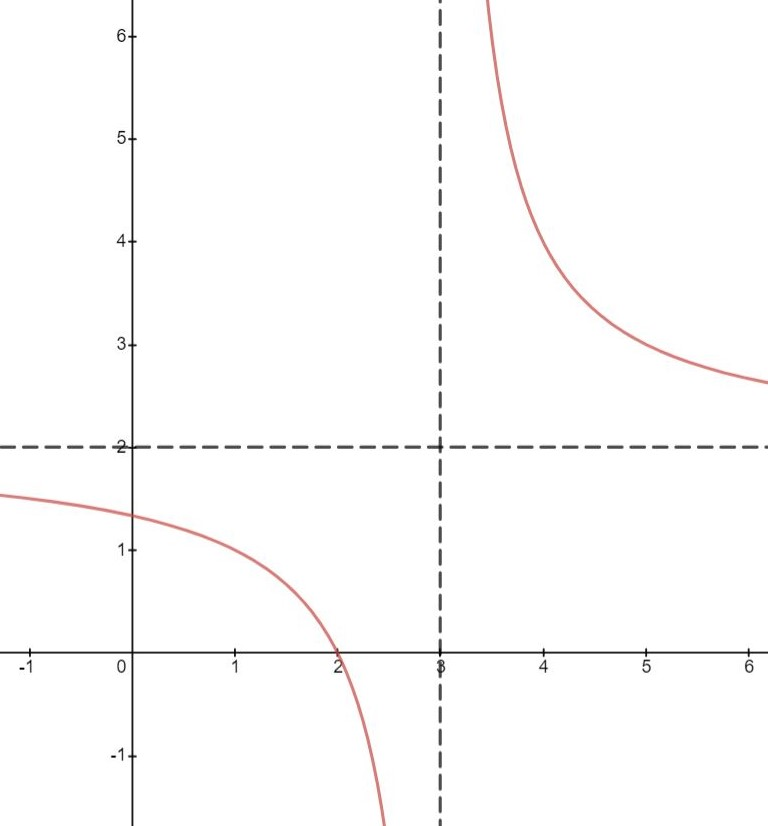
\includegraphics[scale=0.4]{fig1.JPG}}
        \caption{$f(x) = \frac{2x-4}{x-3}$}
        \label{fig:limasymptote}
    \end{center}
\end{figure}

\subsection{Limit Properties}
The limits of combined functions can be found by finding the limit of each of the individual functions, then applying the operations. All the following examples will be based on \hyperref[fig:limasymptote]{Figure 2}.

\begin{itemize}
    \item \textbf{Addition/Subtraction:}

          When taking the limit of the sum or difference of multiple functions, it's the same thing as taking the sum or difference of each of the separate limits or each function.

          \begin{align*}
               & \lim_{x \to 2} \left[ f(x) + g(x) \right]   \\
               & = \lim_{x \to 2} f(x) + \lim_{x \to 2} g(x) \\
               & = 0 + 1                                     \\
               & = 1
          \end{align*}

          \begin{align*}
               & \lim_{x \to 2} \left[ g(x) - f(x) \right]   \\
               & = \lim_{x \to 2} g(x) - \lim_{x \to 2} f(x) \\
               & = 1 - 0                                     \\
               & = 1
          \end{align*}

          \begin{align*}
               & \lim_{x \to 4} \left[ f(x) + g(x) \right]   \\
               & = \lim_{x \to 4} f(x) + \lim_{x \to 4} g(x) \\
               & = \text{undef} + 0                          \\
               & = \text{undef}
          \end{align*}

          \indent Note that in the above equation, because the right and left side limits of $f(x)$ are not the same, its limit is \textit{undefined}. If just one of the functions has an undefined limit, the combined limit would also be undefined.

          \noindent\textbf{The extended Sum Rule:}
          \begin{equation*}
              \lim_{x \to c} \left[ f_1(x) + \cdots + f_n(x) \right]
              = \lim_{x \to c} f_1(x) + \cdots + \lim_{x \to c} f_n(x).
          \end{equation*}
          \smallskip

    \item \textbf{Multiplication:}

          Multiplication of the limits of functions is quite straightforward.

          \begin{align*}
               & \lim_{x \to 2} \left[ f(x) \cdot g(x) \right]   \\
               & = \lim_{x \to 2} f(x) \cdot \lim_{x \to 2} g(x) \\
               & = 0 \cdot 2                                     \\
               & = 0
          \end{align*}

          \indent The same exception applies when one of the limits is \textit{undefined}. This just makes the entire combined limit undefined.

          \noindent\textbf{The extended Product Rule:}
          \begin{equation*}
              \lim_{x \to c} \left[ f_1(x) f_2(x) \cdots f_n(x) \right]
              = \lim_{x \to c} f_1(x) \cdot \lim_{x \to c} f_2(x)
              \cdots f_n(x).
          \end{equation*}
          \smallskip

    \item \textbf{Division:}

          Division is once again basically the same as the other basic operations. There's only one exception, when the denominator is $0$.

          \begin{align*}
               & \lim_{x \to 2} \frac{g(x)}{f(x)}                  \\
               & = \frac{\lim_{x \to 2} g(x)}{\lim_{x \to 2} f(x)} \\
               & = \frac{1}{0}                                     \\
               & = \text{undef}
          \end{align*}

          \noindent\textbf{General quotient rule:}
          \[ \lim_{x \to c} \frac{f(x)}{g(x)} = \frac{\lim_{x \to c} f(x)}{\lim_{x \to c} g(x)}, \quad \textrm{iff} \quad \lim_{x \to c} g(x) \ne 0 \]
          \smallskip

    \item \textbf{Composite Functions:}

          When working with limits of composite functions, it's the same thing as taking the limit of the inner function, then just evaluating the outer function normally.
          \begin{align*}
               & \lim_{x \to 1} f\left(g(x)\right)     \\
               & = f\left( \lim_{x \to 1} g(x) \right) \\
               & = f(2)                                \\
               & = 0
          \end{align*}

          If the limit of the inner function is undefined, the entire equation would also be undefined.
          \begin{align*}
               & \lim_{x \to 4} g\left( f(x) \right)   \\
               & = g\left( \lim_{x \to 4} f(x) \right) \\
               & = g(\text{undef})                     \\
               & = \text{undef}
          \end{align*}
          \smallskip

    \item \textbf{Other Theorems:}

          Given that $\lim f(x)$ and $\lim g(x)$ are both finite for all numbers, and $C$ is a constant:
          \[ \lim k f(x) = k \lim f(x) \]
          \[ \lim_{x \to a} C = C \]
          \smallskip
\end{itemize}

\begin{figure}[H]
    \begin{center}
        \frame{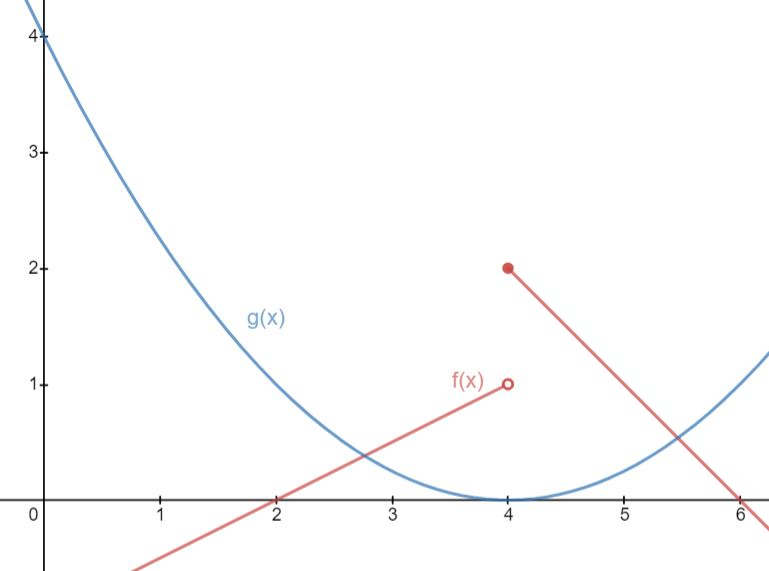
\includegraphics[scale=0.5]{fig2.JPG}}
        \caption[Figure 2]{}
        \label{fig:limproperties}
    \end{center}
\end{figure}

\subsection{Solving Limits}
The first thing to always try when solving limits is \textbf{direct substitution}. If this does not work (undefined limit, 0 as denominator, etc.), then algebraic manipulation (factoring) is the next step.

\begin{align*}
     & \lim_{x \to 2} \frac{x^4 + 3x^3 - 10x^2}{x^2 - 2x}           \\[6pt]
     & = \lim_{x \to 2} \frac{x^2\left[ (x+5)(x-2) \right]}{x(x-2)} \\
     & = \lim_{x \to 2} x(x+5)                                      \\
     & = 14
\end{align*}

\noindent When encountering radicals, conjugates can be used.

\begin{align*}
     & \lim_{x \to -4} \frac{x+4}{\sqrt{3x+13}-1}                                               \\[6pt]
     & = \lim_{x \to -4} \frac{x+4}{\sqrt{3x+13}-1} \cdot \frac{\sqrt{3x+13}+1}{\sqrt{3x+13}+1} \\[6pt]
     & = \lim_{x \to -4} \frac{(\sqrt{3x+13}+1)(\sqrt{3x+13}+1)}{3x+13-1}                       \\[6pt]
     & = \lim_{x \to -4} \frac{(x+4)(\sqrt{3x+13}+1)}{3(x+4)}                                   \\[6pt]
     & = \lim_{x \to -4} \frac{\sqrt{3x+13}+1}{3}                                               \\[6pt]
     & = \frac{2}{3}
\end{align*}

\noindent When dealing with trigonometric equations, use trig identities (if direct substitution does not work).

\begin{align*}
     & \lim_{x \to \frac{\pi}{2}} \frac{\cot^2(x)}{1-\sin(x)}                                                                                \\[6pt]
     & = \lim_{x \to \frac{\pi}{2}} \frac{\cos^2(x)}{\left( \sin^2(x) \right)\left(1-\sin(x)\right)}                                         \\[6pt]
     & = \lim_{x \to \frac{\pi}{2}} \frac{1-\sin^2(x)}{\left( \sin^2(x) \right)\left(1-\sin(x)\right)} \quad \text{(Pythagorean's Identity)} \\[6pt]
     & = \lim_{x \to \frac{\pi}{2}} \frac{\left( 1+\sin(x) \right)\left( 1-\sin(x) \right)}{\left( \sin(x) \right)\left(1-\sin(x)\right)}    \\[6pt]
     & = \lim_{x \to \frac{\pi}{2}} \frac{1+\sin(x)}{\sin^2(x)} \text{, for } x \ne (2k+1)\frac{\pi}{2}                                      \\[6pt]
     & = 2
\end{align*}

\noindent However, functions can not always be factored, so in that case they will just be undefined.

\begin{align*}
     & \lim_{x \to 1} \frac{2x}{x^2 - 7x + 6} \\[6pt]
     & = \lim_{x \to 1} \frac{2x}{(x-6)(x-1)} \\
     & = \frac{2}{0}                          \\
     & = \text{undef}
\end{align*}

The different results achievable from direct substitution can mean different things. $\frac{k}{0}$ means that the limit does not exist, probably an asymptote. $\frac{0}{0}$ means that the limit is indeterminate, use manipulation and try again.

\subsection{Continuity}
A function is continuous at a point if its right and left hand side limits at that point are the same. In other words, it ``can be drawn without lifting the pencil.''
\[ \lim_{x \to c^-} f(x) = \lim_{x \to c^+} f(x).\]

For a function to be \textit{continuous for all real numbers}, it has to give a real number result for all real number $x$. Basically it's continuous over its \textbf{domain} (horizontal).

\begin{itemize}
    \item $\sqrt{x+4}$ is continuous for all $x \ge -4$.
    \item $\sqrt[5]{x}$ is continuous for all $x \in \mathbb{R}$ (odd roots can handle negatives).
    \item $\ln{x}$ is continuous for all $x \ge 0$.
    \item $\frac{1}{x-3}$ is continuous for $x \ne 3$.
\end{itemize}

\textbf{Removable discontinuity} is a function, where the point of discontinuity can be ``removed,'' and the graph of the new function would be almost identical to the original function.

\noindent Given:
\[ \lim_{x \to c} f(x) = k < \infty, \]
where:
\[ F(x) = \begin{cases}
        f(x) & \text{for } x \ne c \\
        k    & \text{for } x = c,
    \end{cases} \]
then $F(x)$ has removable discontinuity at $k$.

\textbf{Jump discontinuity} is when a part of a graph jumps from one $y$ to another on the same $x$ value. (See $f(x)$ in \hyperref[fig:limproperties]{Figure 2}.)

\textbf{Infinite discontinuity} usually occurs when there is a vertical asymptote, and the discontinuity occurs over the asymptote. Both sides of the asymptote approach that value, but never actually touch, so the function is not continuous.

\subsection{Squeeze Theorem}
When it is hard to find the limit for a function, the squeeze theorem (AKA sandwich theorem) can be used. Basically find two other functions, one on top, and one below, and use the limits of the two functions to ``squeeze'' the limit of the given function.

\noindent Given
\[ f(x) \le g(x) \le h(x) \]
for all $x$ in an open interval that includes $c$, and
\[ \lim_{x \to c} f(x) = \lim_{x \to c} h(x) = L, \]
then,
\[ \lim_{x \to c} g(x) = L. \]
Note that $x$ and $L$ can both be $\pm \infty$.

\noindent \textbf{Example:}
\begin{align*}
     & \text{Problem:}                          &                                  & \lim_{x \to \infty} \frac{\sin{x}}{x} \\[6pt]
     & \text{keep in mind that}                 & -1                               & \le \sin{x} \le 1                     \\
     & \text{divide by $x$}                     & \frac{-1}{x}                     & \le \frac{\sin{x}}{x} \le \frac{1}{x} \\[6pt]
     & \text{take limits of smaller functions } & \lim_{x \to \infty} \frac{-1}{x} & = 0 = \lim_{x \to \infty} \frac{1}{x} \\[6pt]
     & \text{Squeeze Theorem:}                  & \lim_{x \to \infty}              & \frac{\sin{x}}{x} = 0.
\end{align*}

The best way to solve the above problem is to first recognize the easier part of the problem, $\sin{x}$. Then manipulate the entire inequality so the middle function becomes the original problem. Solve limits of the two other functions to solve original limit.

\noindent \textbf{Another example:}
\begin{gather*}
    \lim_{x \to -\infty} \frac{x^2(\sin{x} + \cos^{3}{x})}{(x^2+1)(x-3)} \\[8pt]
    \text{Note that:} \\
    -1 \le \sin{x} \le 1, \\
    \because -1 \le \cos{x} \le {1} \\
    \therefore -1 \le \cos^{3}{x} \le 1 \\
    -2 \le \sin{x} + \cos^{3}{x} \le 2 \\[8pt]
    \text{$x$ is approaching negative $\infty$, so $(x-3) < 0$} \\
    \frac{-2}{x-3} \ge \sin{x} + \cos^{3}{x} \ge \frac{2}{x-3} \\[6pt]
    \frac{2x^2}{(x^2+1)(x-3)} \ge \sin{x} + \cos^{3}{x} \ge \frac{-2x^2}{(x^2+1)(x-3)} \\[10pt]
    \lim_{x \to -\infty}\frac{2x^2}{(x^2+1)(x-3)} = 0 \\[6pt]
    \lim_{x \to -\infty}\frac{-2x^2}{(x^2+1)(x-3)} = 0 \\[6pt]
    \therefore \quad \lim_{x \to -\infty} \frac{x^2(\sin{x} + \cos^{3}{x})}{(x^2+1)(x-3)} = 0
\end{gather*}

\subsection{Intermediate Value Theorem}
Given a \textbf{continuous} segment of a function $f(x)$, let $c \in [a, b]$ and $w$ be in between $f(a)$ and $f(b)$. Then there must be \textbf{at least} on value $c$ such that $f(c) = w$. In short, a continuous line from $a \to b$ must pass through every $x$ and $y$ value in between them. (Refer to \hyperref[fig:intvaltheorem]{Figure 3}.) This goes both ways. If there is a $c$, then there is  $w$. If there is a $w$, then there is $c$.

\begin{figure}[H]
    \begin{center}
        \frame{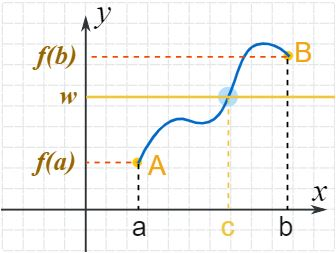
\includegraphics[scale=0.8]{fig3.JPG}}
        \caption{\href{https://www.mathsisfun.com/algebra/intermediate-value-theorem.html}{source}}
        \label{fig:intvaltheorem}
    \end{center}
\end{figure}

\section[Differentiation: Definition and Fundamental Properties (4\% - 7\%)]{Differentiation: Definition and Fundamental \\ (4\% - 7\%)}
\fline

A derivative is the \textbf{instantaneous} rate of change of a function at a point. It's the average rate of change over an infinitely small interval. It has two main notations (names are not important here).
\begin{itemize} % too lazy to keep notation usage uniform across document
    \item \textbf{Lagrange's notation}:
          The derivative of $f(x)$ is $f'(x)$, pronounced ``f prime''. Higher order derivatives are written like $f''(x)$ or $f^2(x)$. In general it's written as $f^{n}(x)$, or with $n$ ticks.
    \item \textbf{Leibniz's notation}:
          The derivative of $f$ is $\frac{d}{dx}$, indicating a derivative with respect to $x$. When $y=f(x)$ the derivative can be written as $\frac{dy}{dx}$. Higher order derivatives are written like $\frac{d^{n}y}{dx^{n}}$.
\end{itemize}

\subsection{Continuity and Differentiability}
\noindent \textbf{Differentiability}: the function must be differentiable for every value in its domain.

\noindent \textbf{Continuity}: the function has no breaks over its domain, ``can be drawn without lifting the pencil.''

\noindent Differentiability \textit{implies} continuity, but continuity does not mean differentiability.

\subsection{Derivative as a Limit}
Not the most useful, but might be on exam. College Board says: ``You'll apply limits to define the derivative.''
\[ \frac{d}{dx} f(x) = \lim_{h \to 0} \frac{f(x+h) - f(x)}{h} \]
\[ \frac{d}{dx} f(a) = \lim_{x \to a} \frac{f(x) - f(a)}{x-a} \]

\noindent \textbf{Example:}
\begin{gather*}
    \text{Derivative of $\sin(x)$ at $x=2$} \\
    \lim_{h \to 0} \frac{f(2+h) - \sin{(2)}}{h} \\
    \text{OR} \\
    \lim_{x \to 2} \frac{\sin{x} - \sin{(2)}}{x-2}
\end{gather*}

\subsection{Differentiation Rules}
\subsubsection{Derivative of a constant}
\noindent The derivative of a constant is always $0$.
\begin{gather*}
    f(x) = C \\
    f'(x) = C' = 0
\end{gather*}

\subsubsection{Constants in a function}
\noindent The constant can be moved outside of the derivative.
\[ \left( k f(x) \right)' = k f'(x) \]

\subsubsection{Sum rule}
The derivative of the sum of many functions is the same as the sum of the derivatives of the individual functions. The same applies for subtraction.
\[ \left[ f_1(x) + f_2(x) + \cdots + f_n(x) \right]' = f'_1(x) + f'_2(x) + \cdots + f'_n(x). \]

\subsubsection{Power Rule}
Simply put the exponent at the front of the variable, then subtract $1$ from the exponent. This also applies to negative or fractional exponents (radicals).
\begin{gather*}
    f(x) = x^p, \; p \in \mathbb{R} \\
    f'(x) = px^{p-1}
\end{gather*}

\subsubsection{Product Rule}
\[ \left[ f(x) \cdot g(x) \right]' = f(x)g'(x) + f'(x)g(x) \]

\subsubsection{Quotient Rule}
\noindent Ho d-hi minus hi d-ho over hoho. (Hi is numerator and ho is denominator.)
\[ \left( \frac{f(x)}{g(x)} \right)' = \frac{f'(x)g(x) - f(x)g'(x)}{g(x)^2} \]

\subsubsection{Chain Rule}
The chain rule allows for the differentiation of a \textit{composition} of two or more function. Take the derivative of the inner function, the multiply that by the derivative of the outer function.
\[ \frac{d}{dx} \left[ f \left( g(x) \right) \right] = f' \left( g(x) \right) g'(x). \]

\noindent Example, derivative of $\sin{x^2}$:
\begin{gather*}
    f(x) = \sin{x} \\
    g(x) = x^2 \\
    \frac{d}{dx} \left[ f \left( g(x) \right) \right] = f' \left( g(x) \right) g'(x) \\
    \frac{d}{dx} \left( \sin{x^2} \right) = \cos{x^2} \; 2x
\end{gather*}

\subsection{Exponential Functions}
Can be solved like the \textbf{chain rule}, with the base and exponent as the outer and inner functions, respectively. The generalized formula is:
\[ \frac{d}{dx} \left( a^x \right) = a^x \ln{a}. \]
The only exception is in $e^x$.
\[ \frac{d}{dx} \left( e^x \right) = e^x.\]

\subsection{Logarithmic Functions}
\noindent The derivative of $\ln{x}$ is:
\[ \frac{d}{dx} \left( \ln{x} \right) = \frac{1}{x}. \]

\noindent This can be used to derive the derivative of other base log functions:
\begin{align*}
    \frac{d}{dx} \left( \log_a{x} \right) & = \frac{d}{dx} \left( \frac{\ln{x}}{\ln{a}} \right)         \\[6pt]
                                          & = \frac{a}{\ln{a}} \cdot \frac{d}{dx} \left( \ln{x} \right) \\[6pt]
                                          & = \frac{1}{\ln{a}} \cdot \frac{1}{x}                        \\[6pt]
    \frac{d}{dx} \left( \log_a{x} \right) & = \frac{1}{x \ln{a}}
\end{align*}

\subsection{Trigonometric Functions}
There really isn't an easy way to memorize these, just try finding patterns. If you do enough problems you'll get to know them better.

Do note that all of the functions other than $\sin$ nas $\cos$ can be derived using the quotient or chain rules.
\begin{center}
    \begin{tabular}{|c|c|}
        \hline
        $f(x)$    & $\frac{dy}{dx}$        \\
        \hline \hline
        $\sin{x}$ & $\cos{x}$              \\
        \hline
        $\cos{x}$ & $-\sin{x}$             \\
        \hline
        $\tan{x}$ & $\frac{1}{\cos^2{x}}$  \\
        \hline \hline
        $\cot{x}$ & $-\frac{1}{\sin^2{x}}$ \\
        \hline
        $\sec{x}$ & $\tan{x} \sec{x}$      \\
        \hline
        $\csc{x}$ & $-\cot{x} \csc{x}$     \\
        \hline
    \end{tabular}
\end{center}

\section{Differentiation: Composite, Implicit, and Inverse Functions (4\% - 7\%)}
\fline
\subsection{Implicit Differentiation}
Implicit differentiation is taking the derivative of both sides of an equation with respect to two variables, usually $x$ and $y$, by treating one variable as a function of the other. (Usually $y$ is a function of $x$.)

\noindent Example:
\begin{align*}
    x^2 + y^2                                                         & = 1            \\
    \frac{d}{dx} \left( x^2 + y^2 \right)                             & = \frac{d}{dx} \\[6pt]
    \frac{d}{dx} \left( x^2 \right) + \frac{d}{dx} \left( y^2 \right) & = 0            \\[6pt]
    2x + 2y \cdot \frac{dy}{dx}                                       & = 0            \\[6pt]
    x + y \cdot \frac{dy}{dx}                                         & = 0            \\[6pt]
    \frac{dy}{dx}                                                     & = -\frac{x}{y}
\end{align*}

When taking the derivative of $y^2$, multiply by $\frac{dy}{dx}$ because the equation is being taken \textbf{as a function of} $x$.

\subsection{Inverse Functions}
\noindent The following formula can be derived using the chain rule:
\begin{gather*}
    g(x) = f^{-1}(x) \\
    g'(x) = \frac{1}{f'\left( g(x) \right)}.
\end{gather*}

\noindent Example, find $(f^{-1})'(1)$:
\begin{align*}
    f(x) = e^x   & \Rightarrow f^{-1}(x) = \ln{x}          \\
    f'(x)        & = e^x                                   \\
    (f^{-1})'(x) & = \frac{1}{f' \left( f^{-1}(x) \right)} \\[6pt]
                 & = \frac{1}{f'(\ln{x})}                  \\[6pt]
                 & = \frac{1}{f'(\ln{(1)})}                \\[6pt]
                 & = \frac{1}{e^{\ln{(1)}}}                \\[6pt]
                 & = \frac{1}{1}                           \\[6pt]
    (f^{-1})'(x) & = 1
\end{align*}

\subsection{Inverse Trigonometric Functions}
These equations can be found using implicit differentiation along with trig identities. \textit{An in depth explanation for each is under the table.}
\begin{center}
    \begin{tabular}{|c|c|}
        \hline
        $f(x)$       & $\frac{d}{dx}$            \\
        \hline \hline
        $\arcsin(x)$ & $\frac{1}{\sqrt{1-x^2}}$  \\
        \hline
        $\arccos(x)$ & $-\frac{1}{\sqrt{1-x^2}}$ \\
        \hline
        $\arctan(x)$ & $\frac{1}{1+x^2}$         \\
        \hline
    \end{tabular}
\end{center}

For the following explanations, keep in mind the \hypertarget{invdertrig}{Pythagorean Identity}, $\sin^2{x} + \cos^2{x} = 1$.
\begin{itemize}
    \item $\arcsin{x}$
          \begin{align*}
              y = \arcsin{x} \;                   & \Rightarrow \; x = \sin{y}                                              \\
              \frac{d}{dx} \left( \sin{y} \right) & = \frac{d}{dx}(x)                                                       \\[6pt]
              (\cos{y}) \frac{dy}{dx}             & = 1                                                                     \\[6pt]
              \frac{dy}{dx}                       & = \frac{1}{\cos{y}}                                                     \\[6pt]
                                                  & = \frac{1}{\sqrt{1 - \sin^2{y}}} \quad \text{\hyperlink{invdertrig}{*}} \\[6pt]
              \frac{dy}{dx}                       & = \frac{1}{\sqrt{1 - x^2}}
          \end{align*}

    \item $\arccos{x}$
          \begin{align*}
              y = \arccos{x} \;        & \Rightarrow \; x = \cos{y}                                               \\
              \frac{d}{dx} (\cos{y})   & = \frac{d}{dx} (x)                                                       \\[6pt]
              (-\sin{y}) \frac{dy}{dx} & = 1                                                                      \\[6pt]
              \frac{dy}{dx}            & = -\frac{1}{\sin{y}}                                                     \\[6pt]
                                       & = -\frac{1}{\sqrt{1 - \cos^2{y}}} \quad \text{\hyperlink{invdertrig}{*}} \\[6pt]
              \frac{dy}{dx}            & = -\frac{1}{\sqrt{1 - x^2}}
          \end{align*}

    \item $\arctan{x}$
          \begin{align*}
              y = \arctan{x} \;                      & \Rightarrow \; x = \tan{y}                                                                           \\
              \frac{d}{dx} (\tan{y})                 & = \frac{d}{dx} (x)                                                                                   \\[6pt]
              \frac{1}{cos^2{y}} \cdot \frac{dy}{dx} & = 1                                                                                                  \\[6pt]
              \frac{dy}{dx}                          & = \cos^2{y}                                                                                          \\[6pt]
                                                     & = \frac{\cos^2{y}}{\cos^2{y} + \sin^2{y}} \quad \text{\hyperlink{invdertrig}{*\textsuperscript{1}}}  \\[6pt]
                                                     & = \frac{1}{1 + \frac{\sin^2{y}}{\cos^2{y}}} \quad \text{\hyperlink{arctander}{*\textsuperscript{2}}} \\[6pt]
                                                     & = \frac{1}{1 + \tan^2{y}}                                                                            \\[6pt]
              \frac{dy}{dx}                          & = \frac{1}{1 + x^2}
          \end{align*}
          \hypertarget{arctander}{*\textsuperscript{2} Divide top and bottom by $\frac{1}{\cos^2{y}}$.}
\end{itemize}

\subsection{Higher Order Derivatives}
To find higher order derivatives, simply take the derivative of the previous order derivative (also applies to implicit differentiation):
\[ \frac{d^n y}{dx^n} f(x) = \frac{dy}{dx} \left( \frac{d^{n-1}y}{dx^{n-1}} f(x) \right). \]

\noindent Example, find second derivative of $2\cos \left( \frac{x}{2} \right)$:
\begin{align*}
    f(x)   & = 2\cos \left( \frac{x}{2} \right)           \\[6pt]
    f'(x)  & = -\sin \left( \frac{x}{2} \right)           \\[6pt]
    f''(x) & = -\frac{\cos \left( \frac{x}{2} \right)}{2}
\end{align*}

\section[Contextual Applications of Differentiation (6\% - 9\%)]{Contextual Applications of Differentiation \\(6\% - 9\%)}
\fline
%* put an intro here ig? whats supposed to be in the intro idk
% \subsection{Rates of Change (Identifying Relevant Information)}

\subsection{Straight-line motion: position, velocity, and acceleration}
\noindent \textbf{Position} is where something is at a specific time ($x(t)$).

\noindent \textbf{Velocity} is how fast something is moving at a specific time ($v(t)$). It determines which direction the object is headed.
\[ v(t) \begin{cases}
        <0 \; \Rightarrow \; \text{Left}    \\
        =0 \; \Rightarrow \; \text{Neither} \\
        >0 \; \Rightarrow \; \text{Right}
    \end{cases} \]

\noindent \textbf{Acceleration} determines whether the velocity is increasing or decreasing at a specific time. If its sign is the same as the sign of velocity, the object is speeding up. If the two signs are different, the object is slowing down. If acceleration is $0$, the object maintains the same velocity.
\\ The \hyperref[fig:posveloaccel]{cartoon} down below explains this relationship quite well.

\begin{figure}[H]
    \begin{center}
        \frame{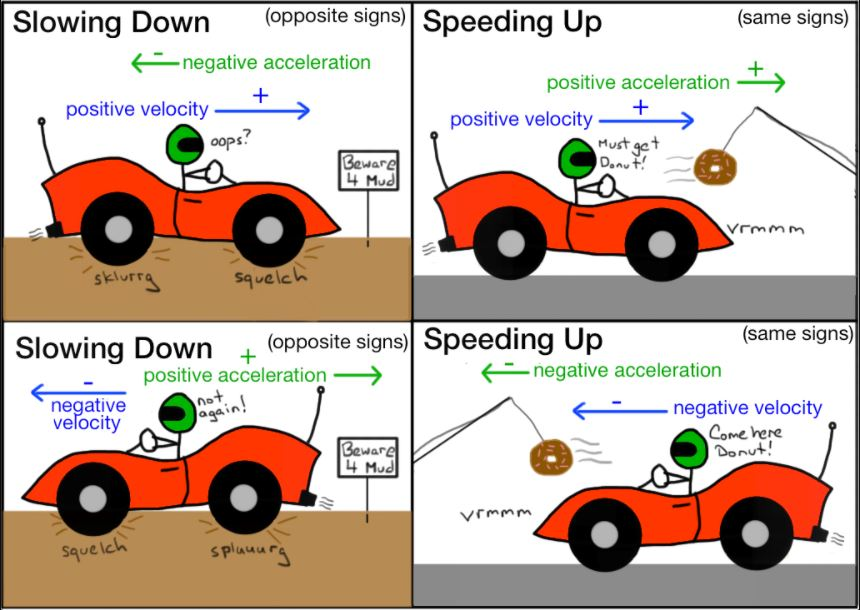
\includegraphics[scale=0.5]{fig4.JPG}}
        \caption{\href{https://www.khanacademy.org/science/physics/one-dimensional-motion/acceleration-tutorial/a/acceleration-article?modal=1}{source}}
        \label{fig:posveloaccel}
    \end{center}
\end{figure}

\begin{center}
    * * * * *
\end{center}

\noindent Position, velocity, and acceleration are related in the following way:
\begin{gather*}
    x'(t) = v(t) \\
    v'(t) = a(t).
\end{gather*}

\subsection{Related Rates}
In simple terms, related rates is using implicit differentiation and given variables to solve for unknown variables. % i feel like more examples should be given in this section. i'm only going to do 2 for now

\noindent Examples:
\begin{enumerate}
    \item Given the equation: $\frac{x}{y} = 9$ and, $\frac{dy}{dt} = -\frac{2}{3}$, \textbf{find} $\frac{dx}{dt}$ \textbf{when} $x=3$.

          \noindent \textbf{Solution}:

          \noindent First differentiate $\frac{x}{y} = 9$ with respect to $t$.
          \begin{align*}
              \frac{x}{y}                                               & = 9 \\[6pt]
              \frac{y \cdot \frac{dx}{dt} - x \cdot \frac{dy}{dt}}{y^2} & = 0
          \end{align*}
          To solve for $\frac{dx}{dt}$, we first have to solve for $y$.
          \begin{align*}
              \frac{x}{y} & = 9           \\[6pt]
              \frac{3}{y} & = 9           \\[6pt]
              y           & = \frac{1}{3}
          \end{align*}
          Finally, plugging in all the variables.
          \begin{align*}
              \frac{y \cdot \frac{dx}{dt} - x \cdot \frac{dy}{dt}}{y^2}                                   & = 0  \\[6pt]
              \frac{\frac{1}{3} \cdot \frac{dx}{dt} - 3 \cdot -\frac{2}{3}}{\left( \frac{1}{3} \right)^2} & = 0  \\[6pt]
              \frac{\frac{dx}{dt} }{3} + 2                                                                & = 0  \\[6pt]
              \frac{\frac{dx}{dt}}{3}                                                                     & = -2 \\[6pt]
              \frac{dx}{dt}                                                                               & = -6
          \end{align*}
          \smallskip

    \item The surface area of a sphere is increasing at a rate of $14 \pi$ square meters per hour. At a certain instant, the surface area is $26 \pi$ square meters. \textbf{What is the rate of change of the volume of the sphere at that instant (in cubic meters per hour)?} (Question from Khan Academy.)

          \noindent \textbf{Solution:}

          \noindent The surface area ($SA$) of a sphere with radius $r$ is $4 \pi r^2$.
          \\ The volume ($V$) of a sphere with radius $r$ is $\frac{4}{3} \pi r^3$.

          \noindent First identify what is given:
          \begin{itemize}
              \item $SA = 36 \pi$
              \item $\frac{dSA}{dt} = 14 \pi$
          \end{itemize}

          \noindent Next, what is unknown:
          \begin{itemize}
              \item $r$, the radius of the sphere.
              \item $\frac{dr}{dt}$, the rate of change of the radius at the instant specified.
              \item $V$, the volume of the sphere (it will be seen later that this is actually not needed, $36 \pi$ if you're curious).
              \item $\frac{dV}{dt}$, the rate of change of the volume at the instant specified (what the question is asking for).
          \end{itemize}

          \noindent Solving for $r$:
          \begin{align*}
              SA     & = 4 \pi r^2 \\
              36 \pi & = 4 \pi r^2 \\
              9      & = r^2       \\
              r      & = 3
          \end{align*}

          \noindent Next, take the derivative of $SA = 4 \pi r^2$ with respect to time, $t$, to solve for the rate of change of $r$ at the instant.
          \begin{align*}
              SA             & = 4 \pi r^2             \\
              \frac{dSA}{dt} & = 8 \pi r \frac{dr}{dt} \\[6pt]
              14 \pi         & = 24 \pi \frac{dr}{dt}  \\[6pt]
              \frac{dr}{dt}  & = \frac{7}{12}
          \end{align*}

          \noindent Finally, take the derivative of $V = \frac{4}{3} \pi r^3$ with respect to time, $t$, to solve for the rate of change of volume.
          \begin{align*}
              V             & = \frac{4}{3} \pi r^3                                                \\[6pt]
              \frac{dV}{dt} & = \frac{4}{3} \pi 3r^2 \frac{dr}{dt}                                 \\[6pt]
                            & = 4 \pi r^2 \frac{dr}{dt} \quad \text{\hyperlink{relratessphere}{*}} \\[6pt]
                            & = 4 \pi 3^2 \cdot \frac{7}{12}                                       \\[6pt]
              \frac{dV}{dt} & = 21 \pi
          \end{align*}
          \hypertarget{relratessphere}{*}Note that $4 \pi r^2$ also happens to be the surface area of the sphere.
\end{enumerate}

\subsection{Local Linearity and Approximation}
\textbf{Local linearity} is the understanding that if we zoom in really, really close to a point on a graph that is differentiable on all points in its domain, it would eventually be a straight line, \textit{the tangent line}.

\noindent The general formula for the equation of the tangent line of function $u$ at $x=a$ is:
\[ y=u'(a)(x-a) + u(a). \]

This can be useful in approximating values on a graph that are close to another, known value. For example, in \hyperref[fig:locallinapprox]{Figure 5}, point A is at $\sqrt{0.25} = 0.5$. Point B is at $\sqrt{0.3}$, which is a bit harder to calculate. But it can be observed that the tangent line at $x=0.25$ comes really close in $y$ value to point B. If the equation of the tangent line was calculated, we could approximate point B.

\noindent \textbf{Approximating point B in \hyperref[fig:locallinapprox]{Figure 5}}:

\noindent Point A is at $(0.25, 0.5)$. The slope of the tangent line can be found using differentiation.
\begin{align*}
    f(x)  & = \sqrt{x}            \\
          & = x^{\frac{1}{2}}     \\
    f'(x) & = \frac{1}{2\sqrt{x}}
\end{align*}

\noindent Plugging in all of this into the line equation:
\begin{align*}
    y & = f'(0.25)(x-0.25) + f(0.25) \\
      & = 1(x-0.25) + 0.5            \\
    y & = x+0.25
\end{align*}

\noindent Now plugging in the $x$ value of point B, which is $0.3$:
\begin{align*}
    y & = 0.3 + 0.25 \\
    y & = 0.55
\end{align*}

The approximation for point B is $(0.3, 0.55)$. Using a calculator, the real value of B is $(0.3, 0.5477)$, which is really close.

\begin{figure}[h]
    \begin{center}
        \frame{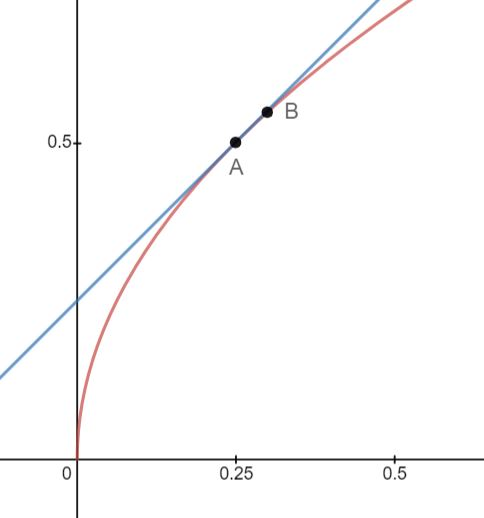
\includegraphics[scale=0.5]{fig5.JPG}}
        \caption{the red (curved) line is $\sqrt{x}$, with its blue tangent line at $x=0.25$.}
        \label{fig:locallinapprox}
    \end{center}
\end{figure}

Another example of this, in a more similar formatting to what would be on an AP exam:

\noindent Let $g$ be a differentiable function with $g(4) = 6$ and $g'(4) = -2$. \textbf{What is the value of the approximation of $g(4.2)$ using the function's local linear approximation at $x=4$?}

\begin{center}
    Plug all of the given information into the line equation formula.
    \begin{align*}
        y & = g'(4)(x-4) + g(4) \\
          & = -2(x-4) + 6       \\
          & = -2x + 8 + 6       \\
        y & = -2x + 14
    \end{align*}

    Now solve with $x=4.2$:
    \begin{align*}
        y & = -2 \cdot 4.2 + 14 \\
          & = -8.4 + 14         \\
        y & = 5.6
    \end{align*}
\end{center}

\subsection{L'Hôpital's Rule} % some spellings say l'hospital
\noindent L'Hôpital's Rule states the following:
\begin{gather*}
    \text{IF} \\
    \lim_{x \to c} \frac{f(x)}{g(x)} = \frac{0}{0} \quad \text{OR} \quad \lim_{x \to c} \frac{f(x)}{g(x)} = \frac{\pm \infty}{\pm \infty} \\[6pt]
    \text{THEN} \\
    \lim_{x \to c} \frac{f(x)}{g(x)} = \lim_{x \to c} \frac{f'(x)}{g'(x)}
\end{gather*}

\noindent Examples:
\begin{enumerate}
    \item Indeterminate form $\frac{0}{0}$:
          \begin{gather*}
              \lim_{x \to 0} \frac{\sin{x}}{x} = \frac{0}{0} \\[6pt]
              \text{Take the derivative of the top and bottom (separately).}\\
              \text{According to L'Hopital's rule:} \\
              \lim_{x \to 0} \frac{\sin{x}}{x} = \lim_{x \to 0} \frac{\cos{x}}{1} \\[6pt]
              = \frac{1}{1} \\[6pt]
              = 1
          \end{gather*}

    \item Indeterminate form $\frac{\infty}{\infty}$: $\lim_{x \to \infty} \frac{e^x}{x^2}$
          \begin{gather*}
              \lim_{x \to \infty} \frac{e^x}{x^2} = \frac{\infty}{\infty} \\[6pt]
              \text{Take the derivative of the top and bottom (separately).}\\
              \text{According to L'Hopital's rule:} \\
              \lim_{x \to \infty} \frac{e^x}{x^2} = \lim_{x \to \infty} \frac{e^x}{2x} \\[6pt]
              \lim_{x \to \infty} \frac{e^x}{2x} = \frac{\infty}{\infty} \\[6pt]
              \text{Apply L'Hopital's rule again:} \\
              \lim_{x \to \infty} \frac{e^x}{2x} = \lim_{x \to \infty} \frac{e^x}{2} \\[6pt]
              = \frac{\infty}{2} \\[6pt]
              = \infty
          \end{gather*}
\end{enumerate}

\section{Analytical Applications of Differentiation}
\fline
%* intro here?
\subsection{Mean Value Theorem}
\begin{wrapfigure}[11]{r}{0.5\textwidth}
    \begin{center}
        \frame{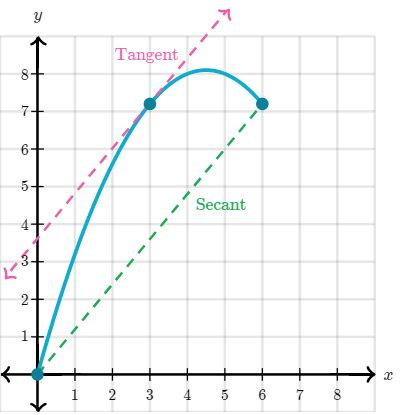
\includegraphics[scale=0.6]{fig6.JPG}}
    \end{center}
    \caption{\href{https://www.khanacademy.org/math/ap-calculus-bc/bc-diff-analytical-applications-new/bc-5-1/a/mean-value-theorem-review?modal=1}{source}}
    \label{fig:meanvaluetheorem}
\end{wrapfigure}

The mean value theorem states that for any arc between two endpoints on a graph, there will be a point whose tangent line will be parallel to the secant line between the two endpoints.

More precisely, given a \textbf{continuous and differentiable} function $f$, in the interval $[a, b]$, there exists a number $c$ such that $f'(c)$ is equal to the average rate of change over $[a, b]$.

\begin{equation*}
    \hspace*{-85mm}
    f'(c) = \frac{f(b)-f(a)}{b-a}
\end{equation*}

\noindent \textit{See \hyperref[fig:meanvaluetheorem]{Figure 6}.}

\subsection{Extreme Value Theorem}
If $f(x)$ is a continuous function over the closed interval $[a, b]$, then there exists a maximum and minimum value of $f(x)$. More formally, there must exist numbers $c$ and $d$ in $[a, b]$ such that:
\[ f(c) \le f(x) \le f(d) \quad \forall x \in [a, b] \]
($\forall$ means for all.)

\subsection[First Derivative Test, Second Derivative Test, and Candidates Test]{First Derivative Test, Second Derivative Test, \\and Candidates Test}
The first derivative test, second derivative test, and candidates test are used together to find relative (local) and absolute (global) extremum in a function.

\subsubsection{Relative (Local) Extrema}
A \textbf{relative maximum} is a point where the value of the function is largest. The direction changes from increasing to decreasing (highest point).

Similarly, a \textbf{relative minimum} is a point where the value of the function is smallest. The direction changes from decreasing to increasing (lowest point).

\noindent \textbf{Using the first derivative test:}

Critical points are points where the derivative of the function is $0$ or undefined. At critical points, there is either an extrema or a point of inflection. For now, we are only concerned with extrema.

\noindent \textbf{Example:} finding the relative extremum of $f(x) = \frac{x^2}{x-1}$.
\begin{align*}
    f(x)  & = \frac{x^2}{x-1}        \\[6pt]
    f'(x) & = \frac{x^2-2x}{(x-1)^2}
\end{align*}
Find the points where $f'(x)$ is $0$ or undefined:
\begin{center}
    \begin{tabular}{|c|c|}
        \hline
        $x$    & $f'(x)$ \\
        \hline \hline
        $0, 2$ & $0$     \\
        \hline
        $1$    & undef   \\
        \hline
    \end{tabular}
\end{center}

Next, test the intervals between the critical points to see whether the function is increasing or decreasing. Simply pick a random number in the interval and see if the derivative is positive or negative at that number.
\begin{center}
    \begin{tabular}{|c|c|c|}
        \hline
        Interval       & $f'(x)$ & Slope of $f(x)$ \\
        \hline \hline
        $(-\infty, 0)$ & $+$     & $\nearrow$      \\
        \hline
        $(0, 1)$       & $-$     & $\searrow$      \\
        \hline
        $(1, 2)$       & $-$     & $\searrow$      \\
        \hline
        $(2, \infty)$  & $+$     & $\nearrow$      \\
        \hline
    \end{tabular}
\end{center}

At $x=0$, $f'(x)$ switches from positive to negative, so $f(x)$ has a relative maximum. Similarly, at $x=2$, $f'(x)$ switches from negative to positive, so $f(x)$ has a relative minimum.

\noindent \textbf{Using the second derivative test:}

The second derivative test can make it a lot easier to determine if a critical point is a maximum or minimum.

\noindent Given
\[ f'(x) = 0, \]
then:
\[ f''(x) \begin{cases}
        >0 \; \Rightarrow \; \text{Minimum point at $x$} \\
        <0 \; \Rightarrow \; \text{Maximum point at $x$} \\
        =0 \; \Rightarrow \; \text{Test is inconclusive}
    \end{cases} \]

One way to remember this is that when $f$ reaches a maximum point, its slope gradually decreases, before reaching $0$ then becoming negative. The slope of the first derivative is the second derivative, so if $f'(x)$ is decreasing, $f''(x)$ is negative. Vice versa for a minimum point.

\subsubsection{Absolute (Global) Extrema}
An absolute extrema is a point on a function where it achieves its greatest or least possible value. Finding the absolute extrema is very similar to finding the relative extrema. The only extra thing to consider are the endpoints of the given interval. (Interval can be entire domain.)

\noindent \textbf{Example (closed domain):}

\noindent Find the global extrema of $f(x) = x^3+2x^2$ over the interval $-2 \le x \le 1$ (\hyperref[fig:absextremaclosed]{Figure 7}).

\noindent Using the first derivative test to find critical points:
\begin{gather*}
    f(x) = x^3 + 2x^2 \\
    f'(x) = 3x^2 + 4x
\end{gather*}
Find the points where $f'(x)$ is $0$ or undefined:
\begin{center}
    \begin{tabular}{|c|c|}
        \hline
        $x$               & $f'(x)$ \\
        \hline \hline
        $-\frac{4}{3}, 0$ & $0$     \\
        \hline
    \end{tabular}
\end{center}
Next, test the intervals between the endpoints and critical points to see whether they are increasing or decreasing.
\begin{center}
    \begin{tabular}{|c|c|c|}
        \hline
        Interval             & $f'(x)$ & Slope of $f(x)$ \\
        \hline \hline
        $(-2, -\frac{4}{3})$ & $+$     & $\nearrow$      \\
        \hline
        $(-\frac{4}{3}, 0)$  & $-$     & $\searrow$      \\
        \hline
        $(0, 1)$             & $+$     & $\nearrow$      \\
        \hline
    \end{tabular}
\end{center}
Over the closed interval, $(-2, 0)$ and $(0, 0)$ are the relative minimums and $(-\frac{4}{3}, 1.185)$ and $(1, 3)$ are the relative maximums.

\noindent \textbf{Both $(-2, 0)$ and $(0, 0)$ have the same $y$ value, so they are both absolute minimums. $(1, 3)$ has the greatest $y$ value so it's the absolute maximum.}
\begin{figure}[H]
    \begin{center}
        \frame{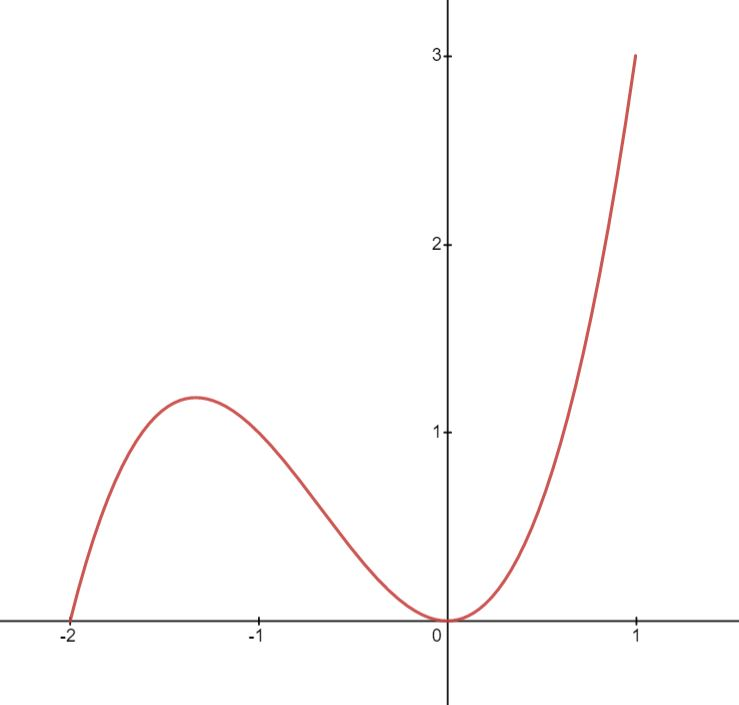
\includegraphics[scale=0.4]{fig7.JPG}}
        \caption{$f(x) = x^3 + 2x^2 \; \{-2 \le x \le 1 \}$}
        \label{fig:absextremaclosed}
    \end{center}
\end{figure}

\subsubsection{Concavity and Points of Inflection}
Concavity is the sign of curvature of a function. Parts of a graph can either be \textit{concave up} or \textit{concave down}. When the concavity is concave up, the first derivative is increasing, thus the second derivative is positive. When the concavity is concave down, the first derivative is decreasing, thus the second derivative is negative.

Inflection points are where the concavity flips. At inflection points both the first and second derivatives are $0$.

\noindent \textbf{Note: when checking if a candidate is an inflection point, the second derivative must change signs!}

\begin{figure}[H]
    \begin{center}
        \frame{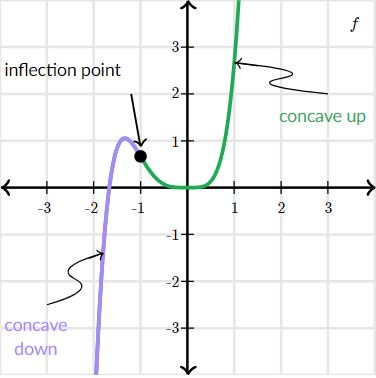
\includegraphics[scale=0.8]{fig8.JPG}}
        \caption{\href{https://www.khanacademy.org/math/ap-calculus-ab/ab-diff-analytical-applications-new/ab-5-6b/a/review-analyzing-the-second-derivative-to-find-inflection-points}{source}}
        \label{fig:concavityinflection}
    \end{center}
\end{figure}

\subsection{Sketching Graphs and Derivatives of Functions} %this is on the college board website, don't know how relevant this is, needs more work
Find maximums, minimums, and points of inflection using first and second derivative tests. It may also be useful to find the zeroes of the function. Then just connect the dots to make the graph.

\subsection{Solving Optimization Problems}
Optimization problems involve finding the largest or smallest something can be. This can be done by first finding a $f(x)$ to represent the relationship, then using $f'(x)$ to find the maximum or minimum.

\noindent \textbf{Examples:}
\begin{enumerate}
    \item Find the $x$ value for which $y=2x+3$ is the closest to the origin.

          \noindent \textbf{Solution:}
          \\ Distance from $(x, y)$ to the origin is:
          \[ D = \sqrt{x^2 + y^2}. \]
          Plug in the given equation:
          \begin{align*}
              D    & = \sqrt{x^2 + y^2}       \\
              D(x) & = \sqrt{x^2 + (2x+3)^2}  \\
                   & = \sqrt{5x^2 + 12x + 9}.
          \end{align*}
          Next, take the derivative of $D(x)$ to find its minimum. It may actually be hard to solve for the $0$s or undefined values of $D'(x)$, so let $L(x) = \left( D(x) \right )^2$. These two functions will have their minimum values at the same $x$, so just take the derivative of $L(x)$ instead.
          \begin{align*}
              L(x)  & = 5x^2 + 12x + 9 \\
              L'(x) & = 10x + 12
          \end{align*}
          Find its critical points where it is $0$ or undefined.
          \begin{align*}
              L'(x)    & = 0            \\
              10x + 12 & = 0            \\
              x        & = -\frac{6}{5}
          \end{align*}
          Use the second derivative test to see if $x=-\frac{6}{5}$ is actually a minimum value.
          \begin{align*}
              L'(x)  & = 10x + 12 \\
              L''(x) & = 10
          \end{align*}
          Because $L''(x)$ is always positive for all $x$, it can be concluded that $x=-\frac{6}{5}$ is indeed a minimum point, and the final answer.

          \begin{center}
              * * * * *
          \end{center}

    \item Find the maximum product of two positive numbers whose sum is $300$.

          \noindent \textbf{Solution:}

          \noindent The question asks to maximize $xy$ given $x+y=300$. The first step is to represent this in a function in terms of $x$, $f(x)$.
          \begin{align*}
              x+y  & = 300        \\
              y    & = 300 - x    \\
              xy   & = x(300-x)   \\
              f(x) & = x(300-x)   \\
                   & = 300x - x^2
          \end{align*}
          Following the same steps as the previous example to find the maximum of $f(x)$:
          \begin{align*}
              f(x)  & = 300x - x^2 \\
              f'(x) & = 300 - 2x.
          \end{align*}
          Find critical points:
          \begin{align*}
              f'(x)    & = 0 \quad \text{(or undefined)} \\
              300 - 2x & = 0                             \\
              x        & = 150.
          \end{align*}
          Second derivative test:
          \begin{align*}
              f'(x)  & = 300 - 2x                            \\
              f''(x) & = -2                                  \\
              f''(x) & < 0 \quad \forall \; x \in \mathbb{R}
          \end{align*}
          Therefore, the $x$ value that yields the maximum product is $150$. Now to find $y$:
          \begin{align*}
              x + y   & = 300 \\
              150 + y & = 300 \\
              y       & = 150
          \end{align*}
          \[ \therefore x=150, \; y=150. \]

          \begin{center}
              * * * * *
          \end{center}

    \item We want to construct a cylindrical can with a bottom but no top that will have a volume of $30$ cm\textsuperscript{3}. Determine the dimensions of the can that will minimize the amount of material needed to construct the can.

          \noindent \textbf{Solution:}
          \begin{gather*}
              V = \pi r^2 h \\
              SA = \pi r^2 + 2\pi rh
          \end{gather*}
          Solve for $h$ to minimize $r$:
          \begin{align*}
              \pi r^2 h & = 30                  \\
              h         & = \frac{30}{\pi r^2}.
          \end{align*}
          Plug this into the $SA$ equation:
          \begin{align*}
              SA(r) & = \pi r^2 + 2\pi r \left( \frac{30}{\pi r^2} \right) \\[6pt]
                    & = \pi r^2 + \frac{60}{r}
          \end{align*}
          Take derivative and find the critical points:
          \begin{gather*}
              SA'(r) = 2 \pi r - \frac{60}{r^2}. \\[6pt]
              \text{Critical points at:} \\
              r = 0, \; \sqrt[3]{\frac{30}{\pi}} \\[6pt]
              \text{*Note that $r=0$ does not exist, as the radius can not be $0$.}
          \end{gather*}
          Second derivative test:
          \begin{gather*}
              SA''(r) = 2 \pi + \frac{120}{r^3} \\[6pt]
              SA'' \left( \sqrt[3]{\frac{30}{\pi}} \right) > 0 \\[6pt]
              \therefore \sqrt[3]{\frac{30}{\pi}} \; \text{is the minimum} \; r.
          \end{gather*}
          Plug $r$ into $h=\frac{30}{\pi r^2}$.

          \noindent Final answer:
          \begin{gather*}
              r = \sqrt[3]{\frac{30}{\pi}} \\[6pt]
              h \approx 2.1215.
          \end{gather*}
\end{enumerate}

\subsection{Behaviors of Implicit Relations} % x and y values in original equation and derivative go back and forth? what's a good way to explain this...
Implicit relations can be useful in solving for unknown values or line equations. The key takeaway is that the variables used in the original function can be substituted back and forth with its higher order derivatives.

\noindent \textbf{Examples:}
\begin{enumerate}
    \item Consider the curve given by $x^3 + xy = -2$. It can be shown that $\frac{dy}{dx} = \frac{-3x^2 - y}{x}$.

          Find the point where the tangent line of the curve is horizontal.
          \bigskip

          \textbf{Solution:}

          For the tangent line to be horizontal, the slope has to be $0$. This means that the numerator of $\frac{dy}{dx}$ must be $0$, but the denominator can not be $0$. Simply solve the system of equations:
          \[ \begin{cases}
                  x^3 + xy = -2 \\
                  -3x^2 - y = 0 \\
                  x \ne 0.
              \end{cases} \]
          \begin{align*}
              -3x^2 - y      & = 0       \\
              y              & = -3x^2   \\[6pt]
              x^3 + x(-3x^2) & = -2      \\
              x^3 - 3x^3     & = -2      \\
              -2x^3          & = -2      \\
              x              & = 1       \\[6pt]
              y              & = -3(1)^2 \\
                             & = -3
          \end{align*}
          Therefore, at $(1, -3)$, the slope of the tangent line is $0$, and thus it is horizontal.
\end{enumerate}

\section{Integration and Accumulation of Change (17\% - 20\%)}
\fline

The accumulation of change is the net change of a quantity. This is not the same thing as simply the quantity. The accumulation of change takes into consideration time, and it is the quantity over a specified time period. There may be some quantity before or after this time period, but we would not count that.

\subsection{Riemann Sums}
A Riemann Sum can be used to approximate the area under a curve. It splits up the area into several rectangles, where the height matches up with the function. The sum of the areas of the rectangles provides a somewhat decent approximation of the actual area.

\subsubsection{Types of Riemann Sums}
\begin{itemize}
    \item \textbf{Left Riemann Sums} line up the left side of the rectangle with the curve of the function.
          \begin{figure}[H]
              \begin{center}
                  \frame{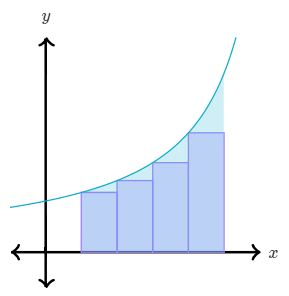
\includegraphics[scale=0.7]{fig9.JPG}}
                  \caption{left Riemann sums, \href{https://www.khanacademy.org/math/ap-calculus-bc/bc-integration-new/bc-6-2/a/riemann-sums-review?modal=1}{source}}
              \end{center}
          \end{figure}

    \item \textbf{Right Riemann Sums} line up the right side of the rectangle with the curve of the function.
          \begin{figure}[H]
              \begin{center}
                  \frame{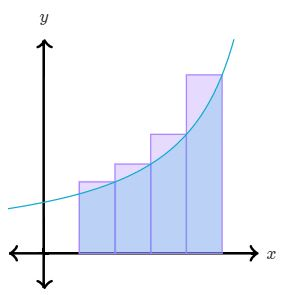
\includegraphics[scale=0.7]{fig10.JPG}}
                  \caption{right Riemann sums, \href{https://www.khanacademy.org/math/ap-calculus-bc/bc-integration-new/bc-6-2/a/riemann-sums-review?modal=1}{source}}
              \end{center}
          \end{figure}

    \item \textbf{Midpoint Riemann Sums} line up the middle of the rectangle with the curve of the function.
          \begin{figure}[H]
              \begin{center}
                  \frame{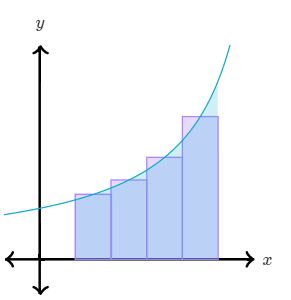
\includegraphics[scale=0.7]{fig11.JPG}}
                  \caption{midpoint Riemann sums, \href{https://www.khanacademy.org/math/ap-calculus-bc/bc-integration-new/bc-6-2/a/riemann-sums-review?modal=1}{source}}
              \end{center}
          \end{figure}

    \item There is another way to approximate areas under a curve, called a \textbf{trapezoidal sum}. Trapezoids are used, and its two bases touch the curve of the function.
          \begin{figure}[H]
              \begin{center}
                  \frame{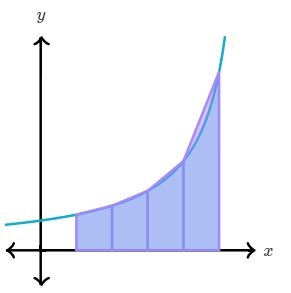
\includegraphics[scale=0.7]{fig12.JPG}}
                  \caption{trapezoidal sums, \href{https://www.khanacademy.org/math/ap-calculus-bc/bc-integration-new/bc-6-2/a/riemann-sums-review?modal=1}{source}}
              \end{center}
          \end{figure}
\end{itemize}

With each type of sum, the more shapes that we have, the closer the approximation would be to the actual area. This can be achieved by making $\Delta x$, the base of the rectangle, smaller and smaller.

\subsubsection{Riemann Sums in Summation Notation}
Given a Riemann sum over the interval $[a, b]$ with $n$ rectangles of equal width, we can define $\Delta x = \frac{b-a}{n}$. The bottom right corner of each rectangle will be $x_i$, so $x_i = a + \Delta x \cdot i$.
\begin{center}
    \begin{tabular}{|c|c|}
        \hline
        Left                                                   & Right                                                \\
        \hline \hline
        $\displaystyle \sum_{i=0}^{n-1} \Delta x \cdot f(x_i)$ & $\displaystyle \sum_{i=1}^{n} \Delta x \cdot f(x_i)$ \\
        \hline
    \end{tabular}
\end{center}

\subsection{Definite Integrals} %* where to include solving definite integrals?
As $\Delta x$ gets smaller and smaller in Riemann Sums, we are able to get better and better approximations of the area under a curve. However, it is impossible to calculate the exact area under the curve using a finite number of rectangles. In order to do so, we need an infinitely small $\Delta x$, or a limit that approaches $0$. Definite integrals can find the \textit{exact} area of an interval under a curve.

\noindent The definite integral notation over the interval $[a, b]$ of $f(x)$ is:
\[ \int_{a}^{b} f(x) \, dx. \]

\noindent The connection between a definite integral and Riemann sum is as follows:
\[ \int_{a}^{b} f(x) \, dx = \lim_{n \to \infty} \sum_{i=1}^{n} \Delta x \cdot f(x_i) \]
where $\Delta x = \frac{b-a}{n}$ and $x_i = a + \Delta x \cdot i$.
\begin{center}
    * * * * *
\end{center}

\textbf{Example of writing definite integral as Riemann sum:}
\[ \int_{\pi}^{2 \pi} \sin(x) \, dx \]
First find $\Delta x$:
\begin{align*}
    \Delta x & = \frac{b-a}{n}         \\[6pt]
             & = \frac{2 \pi - \pi}{n} \\[6pt]
             & = \frac{\pi}{n}.
\end{align*}
Next, find $x_i$:
\begin{align*}
    x_i & = a + \Delta x \cdot i        \\
        & = \pi + \frac{\pi}{n} \cdot i \\[6pt]
        & = \pi + \frac{\pi i}{n}.
\end{align*}
Putting everything together:
\begin{align*}
    \int_{a}^{b} f(x) \, dx          & = \lim_{n \to \infty} \sum_{i=1}^{n} \Delta x \cdot f(x_i)                                           \\[6pt]
    \int_{\pi}^{2 \pi} \sin(x) \, dx & = \lim_{n \to \infty} \sum_{i=1}^{n} \frac{\pi}{n} \cdot \cos{\left( \pi + \frac{\pi i}{n} \right)}.
\end{align*}

\subsection{The Fundamental Theorem of Calculus}
\noindent The fundamental theorem of calculus goes as follows:

\noindent Let $f$ be a function that is continuous over the interval $[a, b]$, and let:
\[ F(x) = \int_{a}^{x} f(t) \, dt. \]
$F$ is the antiderivative of $f$, or in other words, the derivative of $F$ is $f$. This can then tell us how to solve for the area under a curve using antidifferentiation.
\[ \int_{a}^{b} f(x) \, dx = F(b) - F(a) \]

\subsection{Antiderivatives and Integration Techniques}
Antiderivatives are how to get from $f'(x)$ back to $f(x)$. With any antiderivative rule, it can be differentiated and be back to its original function. The antiderivative symbol is just the interval symbol without the defined interval. (Also known as indefinite integrals.)

It is important that we must add a constant (usually represented by $C$), to the end of all antiderivatives. This is because the derivative of \textit{any} constant is $0$. By adding a constant we can consider all possible antiderivatives. % this explanation for C kinda trash

\subsubsection{Reverse Power Rule}
\[ \int x^n \, dx = \frac{x^{n+1}}{n+1} + C\]
\begin{align*}
    \int \sqrt[m]{x^n} \, dx & = \int x^{\frac{n}{m}} \, dx                      \\[6pt]
                             & = \frac{x^{\frac{n}{m} + 1}}{\frac{n}{m} + 1} + C
\end{align*}
\newline
This would also apply to the antiderivative of a constant.
\begin{align*}
    \int A \, dx & = \int Ax^0 \, dx    \\
                 & = \frac{Ax^1}{1} + C \\[6pt]
                 & = Ax + C
\end{align*}

\subsubsection{Reverse Power Rule Exception}
\[ \int \frac{1}{x} \, dx = \ln |x| + C\]

\subsubsection{Exponential Functions}
\[ \int e^x \, dx = e^x + C \]
\[ \int a^x \, dx = \frac{a^x}{\ln(a)} + C \]

\subsubsection{Trigonometric Functions}
\begin{align*}
     & \int \sin(x) \, dx = -\cos(x) + C        \\[6pt]
     & \int \cos(x) \, dx = \sin(x) + C         \\[6pt]
     & \int \sec^2(x) \, dx = \tan(x) + C       \\[6pt]
     & \int \csc^2(x) \, dx = -\cot(x) + C      \\[6pt]
     & \int \sec(x)\tan(x) \, dx = \sec(x) + C  \\[6pt]
     & \int \csc(x)\cot(x) \, dx = -\csc(x) + C
\end{align*}

\subsubsection{Special Case Trigonometric Functions}
\label{sec:arctanintegral}
These integrals may look messy, but they actually are quite common on AP exams. It's useful to recognize these patterns to avoid unnecessary and tedious extra work.
\begin{gather*}
    \int \frac{1}{\sqrt{a^2 - x^2}} \, dx = \arcsin \left( \frac{x}{a} \right) + C \\[6pt]
    \int \frac{1}{\sqrt{a^2 - (bx)^2}} \, dx = \frac{1}{b} \arcsin \left( \frac{bx}{a} \right) + C \\[6pt]
    \int \frac{1}{a^2 + x^2} \, dx = \frac{1}{a} \arctan \left( \frac{x}{a} \right) + C \\[6pt]
    \int \frac{1}{a^2 + (bx)^2} \, dx = \frac{1}{ba} \arctan \left( \frac{bx}{a} \right) + C
\end{gather*}

\subsubsection{Integration by Parts (Products)}
Integration by parts can be used to find the antiderivative of the product of functions. It can also be referred to as the reverse product rule, as it can be derived by rearranging the product rule.
\[ \int f(x) g'(x) \, dx = f(x) g(x) - \int f'(x) g(x) \, dx \]

For integration by parts to be the most useful, $f(x)$ should be a function that is easy to take the derivative of, and $g(x)$ should be a function that is easy to take the antiderivative of.

\noindent For example, find the indefinite integral
\[ \int x \cos(x) \, dx. \]
Let $f(x) = x$ and $g'(x) = \cos(x)$. Next, plug everything in to the equation and solve:
\begin{align*}
    \int x \cos(x) \, dx & = x \sin(x) - \int 1 \cdot \sin(x) \, dx  \\
                         & = x \sin(x) - \left( -\cos(x) \right) + C \\
                         & = x\sin(x) + \cos(x) + C.
\end{align*}

\noindent Another example of this method, find the indefinite integral
\[ \int \ln(x) \, dx. \]
Let $f(x) = \ln(x)$ and $g'(x) = 1$. Therefore, $f'(x) = \frac{1}{x}$ and $g(x) = x$. Plug everything into the equation and solve:
\begin{align*}
    \int \ln(x) \, dx         & = \int \ln(x) \cdot 1 \, dx                       \\
    \int \ln(x) \cdot 1 \, dx & = \ln(x) \cdot x - \int \frac{1}{x} \cdot x \, dx \\[6pt]
                              & = x \ln(x) - \int 1 \, dx                         \\
                              & = x \ln(x) - x + C
\end{align*}

\subsubsection{u-Substitution}
Integration using u-substitution is a very versatile method. In some ways, it can be referred to as the reverse chain rule. It can be used when one part of a function is the derivative of another. A good way to explain this method is through an example.

\noindent Find the indefinite integral:
\[ \int 2x \cos(x^2) \, dx. \]
\newline
Notice that:
\[ \frac{d}{dx} x^2 = 2x. \]
We can apply u-substitution. Let $u = x^2$, then implicitly differentiate:
\begin{align*}
    u              & = x^2                                      \\
    \frac{d}{dx} u & = \frac{d}{dx} x^2                         \\[6pt]
    \frac{du}{dx}  & = 2x                                       \\[6pt]
    du             & = 2x \, dx \quad \hyperlink{eq:usubex1}{*}
\end{align*}
\hypertarget{eq:usubex1}{*}Note that in this step, both sides were multiplied by $dx$. While this is usually unorthodox, it is allowed, and helps in this situation.
\bigskip

\noindent Returning back to the original function, notice that:
\[ \int \cos(\underbrace{x^2}_{u}) \cdot \underbrace{2x \, dx}_{du}. \]
Now substitute and solve:
\begin{align*}
    \int \cos{u} \, du & = \sin{u} + C   \\
                       & = \sin(x^2) + C
\end{align*}
\begin{center}
    * * * * *
\end{center}

Sometimes, we have to multiply the integral by an extra value to make \\u-substitution work. For example, find the definite integral: % \\ to prevent overfull \hbox
\[ \int \sin(3x+5) \, dx. \]
Let $u = 3x+5$, therefore $du = 3 \, dx$. To balance out the $3$ in $du$, we must divide the integral by $3$.
\begin{align*}
    \frac{1}{3} \int \sin{u} \, du & = \frac{1}{3} \left( -\cos(u) \right) + C \\[6pt]
                                   & = -\frac{\cos(3x+5)}{3} + C
\end{align*}

\subsubsection{Partial Fractions} % are these even that necessary
Basically breaking up a fraction into parts to make it easier to antidifferentiate. It is best to explain through an example:

\noindent Find the indefinite integral:
\[ \int \frac{2x+3}{(x+1)(x+2)} \, dx. \]
The fraction can be split up into two parts:
\begin{align*}
    \frac{2x+3}{(x+1)(x+2)} & = \frac{A}{x+1} + \frac{B}{x+2}       \\[6pt]
                            & = \frac{A(x+2) + B(x+1)}{(x+1)(x+2)}.
\end{align*}
Next, solve for $A$ and $B$:
\begin{align*}
    2x+3 & = A(x+2) + B(x+1)  \\
         & = Ax + 2A + Bx + B \\
         & = (A+B)x + 2A + B
\end{align*}
This can be broken down into two equations:
\[ \begin{cases}
        A+B = 2 \\
        2A + B = 3
    \end{cases} \]
\[ \therefore A = 1, \, B = 1 \]
Returning back to the original problem,
\begin{align*}
    \int \frac{2x+3}{(x+1)(x+2)} \, dx & = \int \frac{1}{x+1} + \frac{1}{x+2} \, dx            \\[6pt]
                                       & = \int \frac{1}{x+1} \, dx + \int \frac{1}{x+2} \, dx \\
                                       & = \ln|x+1| + \ln|x+2|
\end{align*}

\subsubsection{Other Integration Methods}
\noindent Some other methods for integration include:

\begin{itemize}
    \item \textbf{Long division}, when encountering a fraction with an equal degree numerator and denominator, just divide. This is the most useful when other methods like u-substitution does not work. For example,
          \[ \frac{2x+7}{x+3} = 2 + \frac{1}{x+3}. \]

    \item \textbf{Completing the square}, when encountering a function that may seem difficult to integrate. By completing the square, we can hopefully rearrange the function to be one that follows a pattern. For example, find the definite integral:
          \[ \int \frac{1}{6x^2+36x+78} \, dx. \]
          First completing the square in the denominator:
          \begin{align*}
              \frac{1}{6x^2+36x+78} & = \frac{1}{6} \cdot \frac{1}{x^2+6x+13}   \\[6pt]
                                    & = \frac{1}{6} \cdot \frac{1}{(x+3)^2 + 4}
          \end{align*}
          Notice that this function now resembles the function that integrates into an $\arctan$ (\hyperref[sec:arctanintegral]{see here}).
          \begin{align*}
              \int \frac{1}{6x^2+36x+78} \, dx & = \int \frac{1}{6} \cdot \frac{1}{(x+3)^2 + 4} \, dx                 \\[6pt]
                                               & = \frac{1}{6} \int \frac{1}{(x+3)^2 + 2^2} \, dx                     \\[6pt]
                                               & = \frac{1}{6} \cdot \frac{1}{2} \arctan \left( \frac{x+3}{2} \right) \\[6pt]
                                               & = \frac{1}{12} \arctan \left( \frac{x+3}{2} \right)
          \end{align*}
\end{itemize}

\subsection{Solving Definite Integrals}
Solving definite integrals involves just a few steps. First, antidifferentiate, then find the difference between the upper bound evaluated at the function and the lower bound evaluated at the function.

\noindent \textbf{Example:}
\begin{align*}
    \int_{27}^{-1} -8 \sqrt[3]{x} \, dx & = \left[ -6 \sqrt[3]{x^4} \right]_{27}^{-1}                \\
                                        & = -6 \sqrt[3]{(-1)^4} - \left( -6 \sqrt[3]{(27)^4} \right) \\
                                        & = -6 + 486                                                 \\
                                        & = 480
\end{align*}

If the two endpoints of the interval are the same, then the value of the definite integral would be $0$:
\[ \int_{a}^{a} f(x) \, dx = 0. \]

\subsection{Determining Improper Integrals}
\noindent Improper integrals are definite integrals that do not cover a finite area.

One type of improper integral occurs when at least one of the endpoints is infinity. For example:
\[ \int_{1}^{\infty} \sqrt{x} \, dx \quad OR \quad \lim_{a \to \infty} \int_{1}^{a} \sqrt{x} \, dx. \]

The other type of improper integral occurs when the function is undefined at at least one of the endpoints (asymptote). For example:
\[ \int_{0}^{1} \frac{1}{x} \, dx \quad OR \quad \lim_{a \to 0} \int_{a}^{1} \frac{1}{x} \, dx. \]

When limits evaluate to a finite value, they \textbf{converge}. If they evaluate to infinity, they \textbf{diverge}.

Solving improper integrals is very similar to solving definite integrals, just this time we have to use limits. Examples:
\begin{itemize}
    \item Endpoint at infinity.
          \begin{align*}
              \int_{-1}^{\infty} \frac{1}{x^2} \, dx & = \lim_{a \to \infty} \int_{-1}^{a} \frac{1}{x^2} \, dx                          \\[6pt]
                                                     & = \lim_{a \to \infty} \left[ -\frac{1}{x} \right]_{-1}^{a}                       \\[6pt]
                                                     & = \lim_{a \to \infty} \left( -\frac{1}{-1} - \left( -\frac{1}{a} \right) \right) \\[6pt]
                                                     & = \lim_{a \to \infty} \left( 1 + \frac{1}{a} \right)                             \\[6pt]
                                                     & = 1+0                                                                            \\
                                                     & = 1
          \end{align*}

    \item Undefined endpoint.
          \begin{align*}
              \int_{0}^{5} \frac{1}{\sqrt{x}} \, dx & = \lim_{a \to 0} \int_{a}^{5} \frac{1}{\sqrt{x}} \, dx \\[6pt]
                                                    & = \lim_{a \to 0} \left[ 2\sqrt{x} \right]_{a}^{5}      \\
                                                    & = \lim_{a \to 0} \left( 2\sqrt{5} - 2\sqrt{a} \right)  \\
                                                    & = 2\sqrt{5} - 0                                        \\
                                                    & = 2\sqrt{5}
          \end{align*}
\end{itemize}

\section{Differential Equations (6\% - 9\%)}
\fline

Differential equations involve functions and their derivatives. Unlike algebraic equations who evaluate to numbers or values, differential equations evaluate to a function or class (several) functions.

\subsection{Modelling Differential Equations}
When interpreting words to turn into differential equations, there are a few keywords that should be looked out for. Listed below are some of the more common ones (examples from Khan Academy):

\begin{itemize}
    \item \textbf{Proportional}: means that the rate of change is equal to some constant $k$ multiplied by what the rate of change is proportional to.
          \bigskip

          \noindent A habitat of prairie dogs can support $m$ dogs at most. The habitat's population, $p$, grows proportionally to the product of the current population and the difference between $m$ and $p$.
          \[ \frac{dp}{dt} = kp(m-p) \]

    \item \textbf{Shrinks, decays, melts, decreases, etc}: any word that suggests something is getting smaller, the rate of change would be equal to some constant $k$ multiplied by what the rate of change is proportional to, but negative.
          \bigskip

          \noindent A radioactive material decays at a rate of change proportional to the current amount, $Q$, of the material.
          \[ \frac{dQ}{dt} = -kQ \]

    \item \textbf{Inversely proportional}: means that the rate of change is equal to the inverse of some constant $k$ multiplied by what the rate of change is proportional to.
          \bigskip

          \noindent A chemical is diluted out of a tank by pumping pure water into the tank and pumping the existing solution out of it, so the volume at any time $t$ is $20+2t$. The amount $z$ of chemical in the tank decreases at a rate proportional to $z$ and inversely proportional to the volume of solution in the tank.
          \[ \frac{dz}{dt} = -\frac{kz}{20-2t} \]

    \item \textbf{Fraction of ... }: usually means that the rate of change is equal to some constant $k$ multiplied by one minus what the rate of change is proportional to.
          \bigskip

          \noindent In one kind of chemical reaction, unconverted reactants change into converted reactants. The fraction $a$ of reactants that have been converted increases at a rate proportional to the product of the fraction of converted reactants and the fraction of unconverted reactants.
          \[ \frac{da}{dt} = ka(1-a) \]
\end{itemize}

\subsection{Slope Fields}
Slope fields area away to verify a class of answers to differential equations that are solved explicitly. When the equation is not solvable explicitly, slope fields provide a way to solve them graphically. Slope fields can show all the different slopes of an equation at all different points on a plane. For example, the slope field for the differential equation $\frac{dy}{dx} = \frac{x-2}{y}$ would look like \hyperref[fig:slopefield1]{this}:

\begin{figure}[H]
    \begin{center}
        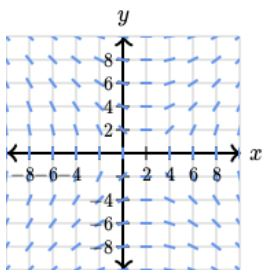
\includegraphics{fig13.JPG}
        \caption{\href{https://www.khanacademy.org/math/ap-calculus-bc/bc-differential-equations-new}{source}}
        \label{fig:slopefield1}
    \end{center}
\end{figure}

We can confirm that this slope field belongs to the above equation by testing a few points. For example:
\begin{itemize}
    \item At $(0, 0)$, $\frac{dy}{dx} = \frac{-2}{0}$, or undefined. This is seen in the slope field by a vertical line, matching the undefined slope.
    \item At $(2, 2)$, $\frac{dy}{dx} = \frac{0}{2}$. This is seen in the slope field by a horizontal line, matching the slope of $0$.
    \item At $(-6, 5)$, $\frac{dy}{dx} = \frac{-8}{5}$. This is seen in the slope field by a line with a negative slope. (It isn't necessary to confirm the slope 100\%, it is sufficient to use an approximation.)
\end{itemize}
% TODO: add more for slope fields maybe

\subsection{Approximation Using Euler's Method}
Euler's method can be used to approximate solutions to otherwise unsolvable differential equations. It's general idea involves solving for $\frac{dy}{dx}$ at one point, then extending the slope over a $\Delta x$, to find the next point to approximate at. At this next point we repeat the steps until we reach the point we hope to achieve.

The steps for approximating the next point given a differential equation and a change in $x$ ($\Delta x$) goes as follows:
\[ f(x_{n+1}) = f(x_n) + \left. \frac{dy}{dx} \right \vert_n \cdot \Delta x. \]

\noindent \textbf{Example:} Given $\frac{dy}{dx} = 2x-3y$ and $f(-1) = 1$, approximate $f(3)$ using $4$ equal steps.

\noindent First, find $\Delta x$.
\begin{align*}
    \Delta x & = \frac{x_n - x_0}{\text{steps}} \\[6pt]
             & = \frac{3-(-1)}{4}               \\[6pt]
             & = 1
\end{align*}
Next, set up a table with what we know so far, using steps of $\Delta x$:
\begin{center}
    \begin{tabular}{|c|c|c|c|}
        \hline
        $n$ & $x$  & $f(x)$ & $\frac{dy}{dx}$ \\
        \hline \hline
        $0$ & $-1$ & $1$    & $-5$            \\
        \hline
        $1$ & $0$  & ?      &                 \\
        \hline
        $2$ & $1$  &        &                 \\
        \hline
        $3$ & $2$  &        &                 \\
        \hline
        $4$ & $3$  &        &                 \\
        \hline
    \end{tabular}
\end{center}
To solve for the value of the box marked by a `?', apply the formula.
\begin{align*}
    f(x_{n+1}) & = f(x_n) + \left. \frac{dy}{dx} \right \vert_n \cdot \Delta x \\[6pt]
    f(x_1)     & = f(x_0) + \left. \frac{dy}{dx} \right \vert_0 \cdot \Delta x \\[6pt]
               & = 1 + (-5) \cdot 1                                            \\
               & = -4
\end{align*}
Rinse and repeat these steps for the remaining of the boxes to fill in the table.
\begin{center}
    \begin{tabular}{|c|c|c|c|}
        \hline
        $n$ & $x$  & $f(x)$ & $\frac{dy}{dx}$ \\
        \hline \hline
        $0$ & $-1$ & $1$    & $-5$            \\
        \hline
        $1$ & $0$  & $-4$   & $12$            \\
        \hline
        $2$ & $1$  & $8$    & $-22$           \\
        \hline
        $3$ & $2$  & $-14$  & $46$            \\
        \hline
        $4$ & $3$  & $32$   &                 \\
        \hline
    \end{tabular}
\end{center}
Using Euler's Method, we have approximated $f(3) = 32$.

\subsection{Separable Differential Equations}
A separable differential means that the variables can be separated. In other words, the $x$'s can be rearranged to be with the other $x$'s, and the $y$'s can be rearranged to be with the other $y$'s. Doing so makes it possible to separately integrate the two sides of the equation.

Note that not all differentiable equations are separable. For an equation to be separable, it must be the product or quotient of $f(x)$ and $g(y)$. For example,
\[ \frac{dy}{dx} = f(x) g(y) \quad \text{or} \quad \frac{dy}{dx} = \frac{g(y)}{f(x)} \]
are separable.

Listed below are a few examples of separable and non-separable differential equations.
\begin{enumerate}
    \item $\frac{dy}{dx} = 3x + 4y$

          This equation is not separable, as it is the sum of two functions.
          \bigskip

    \item $\frac{dy}{dx} = 2^{x-y}$

          This equation is separable. It can be rearranged to be the quotient of a $f(x)$ and a $g(y)$.
          \begin{align*}
              2^{x-y} & = 2^x \cdot 2^{-y} \\
                      & = \frac{2^x}{2^y}.
          \end{align*}

    \item $\frac{dy}{dx} = 5y - x^2 y$

          This equation is separable. It can be factored to be the product of a $f(y)$ and a $g(x)$.
          \[ 5y - x^2 y = y(5-x^2). \]
\end{enumerate}

\subsubsection{General Solutions}
A general solution to a differential equation would take into consideration the entire class of possible solutions. This means that we have to add a constant, $C$, to the end of the function.

\noindent Here is an example:
\[ \frac{dy}{dx} = e^x y^2. \]

The first step would be to separate the equation. This is the same as rearranging the equation into the form of $f(y) \, dy = g(x) \, dx$. Normally, it is not orthodox to separate $dy$ and $dx$ to rearrange them. However, in separable differential equations this is allowed.
\begin{align*}
    \frac{dy}{dx}     & = e^x y^2   \\[6pt]
    y^2 \frac{dy}{dx} & = e^x       \\[6pt]
    y^2 \, dy         & = e^x \, dx
\end{align*}
Next, take the integral of both sides. If the left and right hand sides are equal, their indefinite integrals would also be equal.
\begin{align*}
    \int y^2 \, dy & = \int e^x \, dx \\
    \frac{y^3}{3}  & = e^x + C
\end{align*}
Notice that we only need to add a constant to one side, as adding a constant to both sides would be redundant.

\noindent The final step is to rearrange the equation and solve for $y$.
\begin{align*}
    \frac{y^3}{3} & = e^x + C                            \\[6pt]
    y^3           & = 3 \left( e^x + C \right)           \\
    y             & = \sqrt[3]{3 \left( e^x + C \right)}
\end{align*}

\subsubsection{Particular Solutions}
Particular solutions to differential equations would be solving for the constant, $C$, as well. \textit{Particular} means we are solving for a specific equation, not an entire class of them.

\noindent Here is an example:
\[ f'(x) = \frac{16}{x^2}, \, f(-2) = 0. \]
Find $f(4)$.

The first step is to solve for the class of functions that work for the differential equation.
\begin{align*}
    \frac{dy}{dx} & = \frac{16}{x^2}            \\[6pt]
    dy            & = \frac{16}{x^2} \, dx      \\[6pt]
    \int 1 \, dy  & = \int \frac{16}{x^2} \, dx \\[6pt]
    y             & = -\frac{16}{x} + C
\end{align*}
Next, we can plug in the given value to solve for $C$.
\begin{align*}
    f(-2)              & = 0  \\
    -\frac{16}{-2} + C & = 0  \\[6pt]
    8 + C              & = 0  \\
    C                  & = -8
\end{align*}
This leaves us with the specific function:
\[ f(x) = -\frac{16}{x} - 8. \]
Finally, solve for the unknown $y$ by plugging in its given $x$.
\begin{align*}
    f(4) & = -\frac{16}{4} - 8 \\[6pt]
         & = -4 - 8            \\
         & = -12
\end{align*}

\subsection{Homogeneous Differential Equations}
A homogeneous differential equation is in the form $\frac{dy}{dx} = f \left( \frac{y}{x} \right)$. To solve these, we can make the substitution $v = \frac{y}{x}$.

Implicitly differentiating $v = \frac{y}{x}$ with respect to $x$ (using product rule) gives:

\[ \frac{dy}{dx} = x \frac{dv}{dx} + v .\]

For example:
\[ 4x \frac{dy}{dx} = x + 2y \]

The first step is to rewrite the equation to be a function of $\frac{y}{x}$, by dividing both sides by $4x$.
\[ \frac{dy}{dx} = \frac{1}{4} + \frac{1}{2} \cdot \frac{y}{x}. \]

Next, make the substitutions for $\frac{y}{x}$ and $\frac{dy}{dx}$.
\begin{align*}
    x \frac{dv}{dx} + v & = \frac{1}{4} + \frac{v}{2} \\[6pt]
    x \frac{dv}{dx}     & = \frac{1}{4} - \frac{v}{2}
\end{align*}

Solve the differential equation with $v$ and $x$.
\begin{align*}
    x \frac{dv}{dx}             & = \frac{1}{4} - \frac{v}{2}        \\[6pt]
    x \frac{dv}{dx}             & = \frac{1 - 2v}{4}                 \\[6pt]
    \frac{4}{1 - 2v} \, dv      & = \frac{1}{x} \, dx                \\[6pt]
    \int \frac{4}{1 - 2v} \, dv & = \int \frac{1}{x} \, dx           \\[6pt]
    -2 \ln|1 - 2v|              & = \ln|x| + C                       \\
    \ln|1 - 2v|                 & = -\frac{1}{2} \ln|x| + C          \\[6pt]
    1 - 2v                      & = e^{-\frac{1}{2} \ln|x| + C}      \\[6pt]
    1 - 2v                      & = A e^{\ln x^{-\frac{1}{2}}}       \\[6pt]
    1 - 2v                      & = A x^{-\frac{1}{2}}               \\[6pt]
    v                           & = \frac{1 - A x^{-\frac{1}{2}}}{2} \\[6pt]
\end{align*}

Finally, substitute $\frac{y}{x}$ back into $v$.
\begin{align*}
    \frac{y}{x} & = \frac{1 - A x^{-\frac{1}{2}}}{2}         \\[6pt]
    y           & = x \cdot \frac{1 - A x^{-\frac{1}{2}}}{2}
\end{align*}

\subsection{Integrating Factor}
The integrating factor technique can be used to solve any differential equation in the form:
\[ \frac{dy}{dx} + P(x)y = Q(x). \]

By multiplying the equation by another function, $I(x)$, we notice that the left-hand side of the equation resembles the product rule for implicitly differentiating $I(x) y$:
\[ I(x) \frac{dy}{dx} + I(x) P(x)y = I(x) Q(x). \]

Therefore, we need to find $I(x)$ so that $I'(x) = I(x) P(x)$. This can be done by solving the differential equation with the following steps. Notice that the constant factor is not considered in the integrating step to simplify the final product.
\begin{align*}
    I'(x)           & = I(x) P(x)                     \\
    P(x)            & = \frac{I'(x)}{I(x)}            \\[6pt]
    \int P(x) \, dx & = \int \frac{I'(x)}{I(x)} \, dx \\[6pt]
    \int P(x) \, dx & = \ln|I(x)|                     \\
    I(x)            & = e^{\int P(x) \, dx}
\end{align*}

Altogether, the steps for using the integrating factor technique are as follows:
\begin{enumerate}
    \item Calculate the integrating factor using $I(x) = e^{\int P(x) \, dx}$.
    \item Multiply both sides of the equation by $I(x)$.
    \item Integrate to obtain a general solution.
\end{enumerate}

For example:
\[ \frac{dy}{dx} - 4y = e^x. \]

First, we notice that $P(x) = -4$. Therefore:
\begin{align*}
    I(x) & = e^{\int -4 \, dx} \\
    I(x) & = e^{-4x}
\end{align*}

Multiplying the differential equation by $I(x)$ gives:
\[ e^{-4x} \frac{dy}{dx} - e^{-4x} \cdot 4y = e^x \cdot e^{-4x}. \]

Finally, we can solve for the general solution.
\begin{align*}
    e^{-4x} \frac{dy}{dx} - e^{-4x} \cdot 4y        & = e^x \cdot e^{-4x}         \\[6pt]
    \frac{d}{dx} \left( e^{-4x}y \right)            & = e^{-3x}                   \\[6pt]
    \int \frac{d}{dx} \left( e^{-4x}y \right) \, dx & = \int e^{-3x} \, dx        \\[6pt]
    e^{-4x}y                                        & = -\frac{e^{-3x}}{3} + C    \\[6pt]
    y                                               & = -\frac{e^x}{3} + C e^{4x}
\end{align*}

In this other example, we observe that the equation is already in the form $I(x) \frac{dy}{dx} + I(x) P(x)y = I(x) Q(x)$, with $P(x) = 2x$:
\[ x^2 \frac{dy}{dx} + 2xy = 1. \]

We can solve this by integrating both sides:
\begin{align*}
    \frac{d}{dx} \left( x^2 y \right)            & = 1                 \\[6pt]
    \int \frac{d}{dx} \left( x^2 y \right) \, dx & = \int 1 \, dx      \\[6pt]
    x^2 y                                        & = x + C             \\
    y                                            & = \frac{x + C}{x^2}
\end{align*}

\subsection{Exponential Model Equations}
Exponential model equations means that the differential equation will have to deal with exponents in one way or another. If the equation is separable, it can still be solved in the same way.

\noindent Examples:
\begin{enumerate}
    \item Solve for $g(x)$, given:
          \[ g'(x) = -4 g(x) \, \text{, and} \, g(-2) = 12. \]

          The first step is to find the general solution for $g(x)$.
          \begin{align*}
              g'(x)                  & = -4 g(x)       \\
              \frac{dy}{dx}          & = -4y           \\[6pt]
              \frac{1}{y} \, dy      & = -4 \, dx      \\[6pt]
              \int \frac{1}{y} \, dy & = \int -4 \, dx \\[6pt]
              \ln|y|                 & = -4x + C       \\
              y                      & = e^{-4x + C}
          \end{align*}
          The next step would be to solve for $C$, in order to find the particular solution for $g(x)$. It may be easier to do so if we first rearrange the equation a bit.
          \begin{align*}
              y & = e^{-4x + C}                                               \\
                & = e^{-4x} \cdot e^C                                         \\
                & = C \cdot e^{-4x} \quad \text{\hyperlink{eq:expmodeeq1}{*}}
          \end{align*}
          \hypertarget{eq:expmodeq1}{*}Note that $e$ to the power of an arbitrary constant will still be a constant.
          \begin{align*}
              g(-2)       & = 12                      \\
                          & = C \cdot e^{-4 \cdot -2} \\
              C \cdot e^8 & = 12                      \\
              C           & = 12 e^{-8}
          \end{align*}
          Putting everything together,
          \begin{align*}
              \therefore g(x) & = e^{-4x} \cdot 12 e^{-8} \\
                              & = 12 e^{-4x-8}
          \end{align*}
          \smallskip

    \item The number of barrels of oil a certain company exports annually increases at a rate that is proportional at any time to the number of barrels they export at that time. The company exported $5.4$ million barrels annually initially, and it exported $10.8$ million barrels annually after $6$ years.

          \noindent \textbf{How many million barrels of oil did the company export after $10$ years?} Round your answer to the nearest whole number.

          \vspace{6mm}

          We first have model the differential equation. Let $B$ be the number of millions of barrels of oil, let $t$ be the number of years, and let $k$ be an arbitrary number. The differential equation can be modelled as:
          \[ \frac{dB}{dt} = kB. \]

          We recognize that this is a separable differential equation, so we can solve for $B(t)$.
          \begin{align*}
              \frac{dB}{dt}          & = kB             \\[6pt]
              \frac{1}{B} \, dB      & = k \, dt        \\[6pt]
              \int \frac{1}{B} \, dB & = \int k \, dt   \\[6pt]
              \ln|B|                 & = kt + C         \\
              B(t)                   & = e^{kt + C}     \\
                                     & = C \cdot e^{kt}
          \end{align*}

          We can use the two given values, $B(0) = 5.4$ and $B(6) = 10.8$, to solve for $C$ and $k$.
          \begin{align*}
              B(0)             & = 5.4             \\
              C \cdot e^{0k}   & = 5.4             \\
              C                & = 5.4             \\[10pt]
              B(6)             & = 10.8            \\
              5.4 \cdot e^{6k} & = 10.8            \\
              e^{6k}           & = 2               \\
              6k               & = \ln 2           \\
              k                & = \frac{\ln 2}{6}
          \end{align*}

          Putting everything together and solving for $B(10)$:
          \begin{align*}
              B(t)  & = 5.4 \cdot e^{\frac{\ln 2}{6} t}        \\
              B(10) & = 5.4 \cdot e^{10 \cdot \frac{\ln 2}{6}} \\
                    & \approx 17
          \end{align*}

          The company will be making approximately $17$ million barrels of oil in $10$ years.
\end{enumerate}

\subsection{Logistic Growth Model Equations}
A logistic model is an s-shaped curve that starts by growing rapidly before slowing down as it approaches its \textit{carrying capacity}. It can be used to represent population.

The change in population is proportional to the product of the population at the time, $P$, and the difference between $1$ and the current population, $P$, over the carrying capacity, $C$. (\hyperref[fig:logisticeq]{Figure 14})
\[ \frac{dP}{dt} = kP \left( 1 - \frac{P}{C} \right) \]

\begin{figure}[H]
    \begin{center}
        \frame{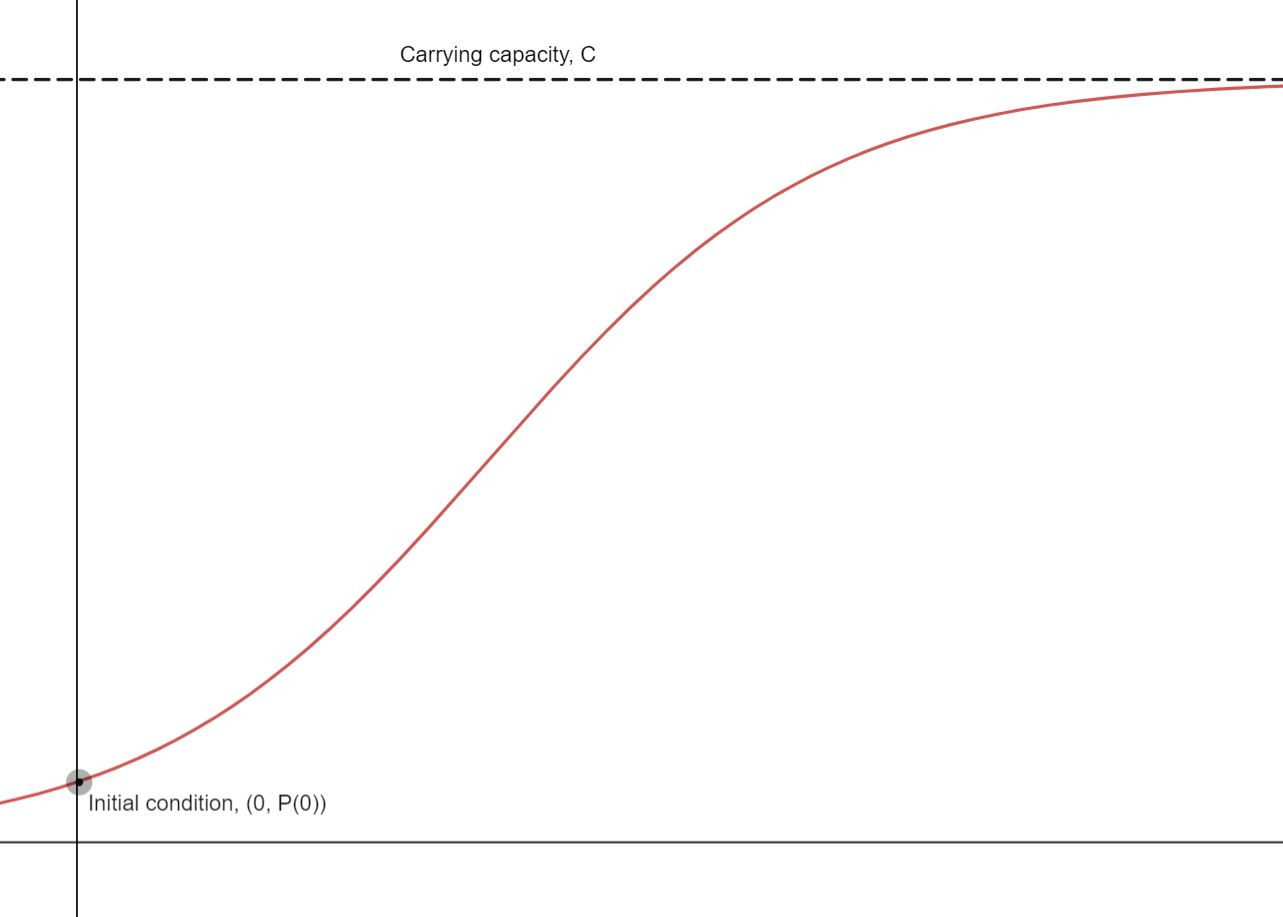
\includegraphics[scale=0.4]{fig14.JPG}}
        \caption{Logistic Equation, $P(t)$}
        \label{fig:logisticeq}
    \end{center}
\end{figure}

\noindent \textbf{Examples:}
\begin{enumerate}
    \item Find the carrying capacity of the following logistic growth:
          \[ \frac{dP}{dt} = \frac{1}{50} P (35000 - P). \]

          For any logistic model $P$, $\frac{dP}{dt}$ will approach $0$ at the carrying capacity.
          \begin{align*}
              \frac{dP}{dt}              & = 0           \\[6pt]
              \frac{1}{50} P (35000 - P) & = 0           \\[6pt]
              P                          & = 0, \, 35000
          \end{align*}
          $P=0$ is the lower limit for $P$, so $P=35000$ is the carrying capacity.
          \bigskip

    \item At what value $N$ does the following logistic model grow the quickest?
          \[ \frac{dN}{dt} = N \left( 0.1 - \frac{N}{1800000} \right) \]

          The point at which the logistic equation grows the quickest would be at its point of inflection. This is when the derivative changes from increasing to decreasing. (When second derivative is $0$.) It can be noticed that the graph of the first derivative is parabolic. In order to find the $N$ value of the maximum of the first derivative, we can find its zeroes then take their average.
          \begin{gather*}
              N \left( 0.1 - \frac{N}{1800000} \right) = 0 \\[6pt]
              N = 0, \, 180000
          \end{gather*}
          Taking the average of the zeroes,
          \begin{align*}
              N & = \frac{0 + 180000}{2} \\[6pt]
                & = 90000
          \end{align*}

          Therefore, the model is growing the quickest at $N=90000$.
\end{enumerate}

\section{Applications of Integration (6\% - 9\%)}
\fline

\subsection{Average of a Function Over an Interval} % are examples needed for this?
The average of a function over an interval is equal to the sum of all its $y$ values divided by the length of the interval. This sum is the same thing as the area under the curve, or the definite integral over the interval.
\[ f_{avg} = \frac{1}{b-a} \int_{a}^{b} f(x) \, dx \]

\subsection{Particle Motion (Position, Velocity and Acceleration)}
Similar to how derivatives can be used to derive velocity from position or acceleration from velocity, integrals can be used to go the other way around.
\begin{gather*}
    \int a(t) = v(t) \\
    \int v(t) = p(t)
\end{gather*}

There are three possible types of problems that involve velocity and position and require integrals.
\begin{itemize}
    \item \textbf{Displacement}

          Displacement is essentially the distance from a particle's starting point to its current position. If it moves forward then back again, it would not count the distance it travelled back.
          \[ \int_{a}^{b} v(x) \, dx \]

    \item \textbf{Total distance}

          Total distance a particle has taken to get from one point to another. If a particle moves forward then back again, it would count both distances.
          \[ \int_{a}^{b} |v(x)| \, dx \]

    \item \textbf{Actual position}

          The actual position is where the particle is at given a specific time, $b$.
          \[ p(b) = v(a) + \int_{a}^{b} v(x) \, dx \]
\end{itemize}

\noindent Example problems:
\begin{enumerate}
    \item A particle with velocity $v(t) = 3\sqrt{t}$, where $t$ is seconds, moves in a straight line. How far does the particle move from $t=1$ to $t=4$?

          This problem is asking for the particle's total distance travelled, as hinted by ``how far does the particle move'' rather than ``how far is the particle from its starting position.''
          \begin{align*}
              \int_{1}^{4} |3\sqrt{t}| \, dx & = \left[ 2 t^{\frac{3}{2}} \right]_{1}^{4} \\
                                             & = 16 - 2                                   \\
                                             & = 14
          \end{align*}
          The particle moves $14$ units from $t=1$ to $t=3$.

    \item As a particle moves along the number line, its position at time $t$ is $s(t)$ its velocity is $v(t)$ and its acceleration is $a(t)= 12t-4$. If $v(2)=4$ and $s(0)=1$, what is $s(1)$.

          The first step in this problem is solving for the particular $v(t)$.
          \begin{align*}
              v(t) & = \int a(t) \, dt  \\[6pt]
                   & = \int 12t-4 \, dt \\
                   & = 6t^2 -4t + C
          \end{align*}
          Solving for $C$:
          \begin{align*}
              v(2)       & = 4            \\
              24 - 8 + C & = 4            \\
              C          & = -12          \\
              v(t)       & = 6t^2 -4t -12
          \end{align*}

          The problem is asking for the actual position of the particle at $t=1$.
          \begin{align*}
              s(1) & = s(0) + \int_{0}^{1} v(t) \, dt               \\[6pt]
                   & = 1 + \int_{0}^{1} 6t^2 -4t -12 \, dt          \\
                   & = 1 + \left[ 2t^3 - 2t^2 - 12t \right]_{0}^{1} \\
                   & = 1 -12 +0                                     \\
                   & = -11
          \end{align*}
          The position of the particle at $t=1$ is $-11$ units.
\end{enumerate} % maybe add more problems later

\subsection{Accumulation Problems}
Accumulation is something's net change, usually a quantity. Given a rate of change, we can find the value using integrals. The net change of a quantity $f(t)$ from time $a$ to $b$ is:
\[ \int_{a}^{b} f'(t) \, dt. \]

This can also be used to find the quantity of something after an interval, giving a starting point.
\[ f(b) = f(a) + \int_{a}^{b} f'(t) \, dt \]

\noindent \textbf{Examples:}
\begin{enumerate}
    \item The water level of a strait is changing at a rate of $\frac{3}{2} \sin \left(2- \frac{t}{2}) \right)$ centimeters per hour (where $t$ is hours since midnight). Approximate how much the water level changes from $t=1$ to $t=3$ (round to nearest whole number).

          Let $r(t) = \frac{3}{2} \sin \left(2- \frac{t}{2}) \right)$. A key point to realize is that this function is the \textit{rate of change} of the water level, not the water level itself. So to find the change in water level we can use:
          \[ \int_{1}^{4} r(t) \, dt. \]

          \begin{align*}
              \int_{1}^{4} \frac{3}{2} \sin \left(2- \frac{t}{2} \right) \, dt & = \left[ 3 \cos \left(2 - \frac{t}{2} \right) \right]_1^4 \\[6pt]
                                                                               & = 3 \cos(0) - 3\cos \left( \frac{3}{2} \right)            \\[6pt]
                                                                               & \approx 2.8
          \end{align*}

          The water level rises by approximately $2.8$ centimetres from $t=1$ to $t=4$.
\end{enumerate} % add more examples later

\subsection{Area Between Curves}
\subsubsection{Curves as Functions of x}
The most basic type of area between a curve is the area under a single curve. The area under the curve $f(x)$ over the interval $[a, b]$ is the same as:
\[ \int_a^b f(x) \, dx. \]
For example, what is the area under the curve of $\cos(x)$ from $0$ to $\frac{\pi}{2}$?
\begin{align*}
    \int_0^{\frac{\pi}{2}} \cos(x) \, dx & = \left[ \sin(x) \right]_0^{\frac{\pi}{2}} \\[6pt]
                                         & = 1 - 0                                    \\
                                         & = 1
\end{align*}
This area is the same as the shaded area in \hyperref[fig:auccosx1]{Figure 15}:

\begin{figure}[H]
    \begin{center}
        \frame{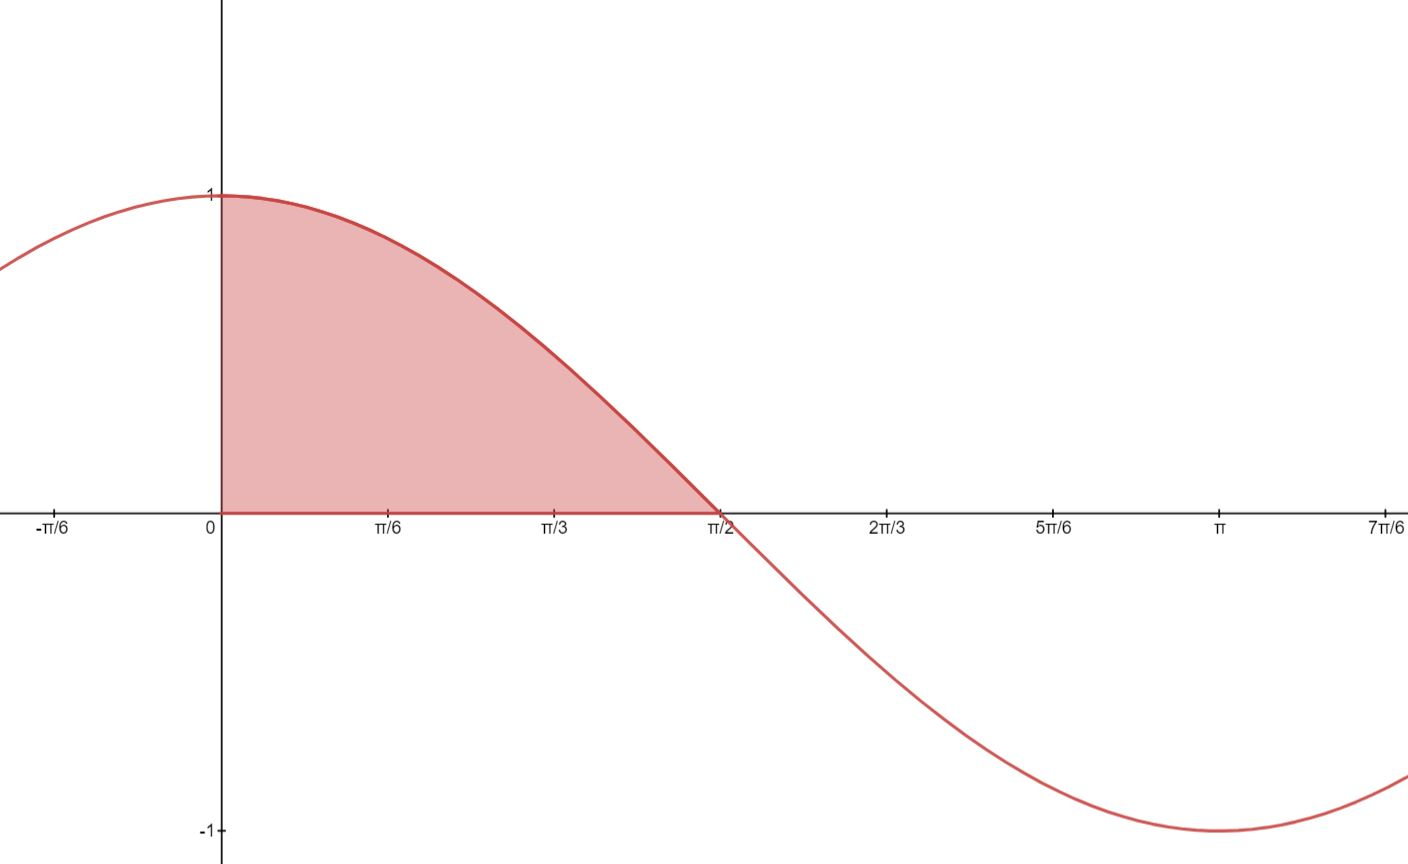
\includegraphics[scale=0.3]{fig15.JPG}}
        \caption{Area under the curve of $\cos(x)$ over $x \in [0, \frac{\pi}{2}]$}
        \label{fig:auccosx1}
    \end{center}
\end{figure}

The area under the curve can also be negative if it is under the $x$ axis. An example of this is the area under the curve of $\cos(x)$ from $\frac{\pi}{2}$ to $\pi$. (See \hyperref[fig:auccosx2]{Figure 16}.)
\begin{align*}
    \int_{\frac{\pi}{2}}^\pi \cos(x) \, dx & = \left[ \sin(x) \right]_{\frac{\pi}{2}}^\pi \\[6pt]
                                           & = 0 - 1                                      \\
                                           & = -1
\end{align*}

\begin{figure}[H]
    \begin{center}
        \frame{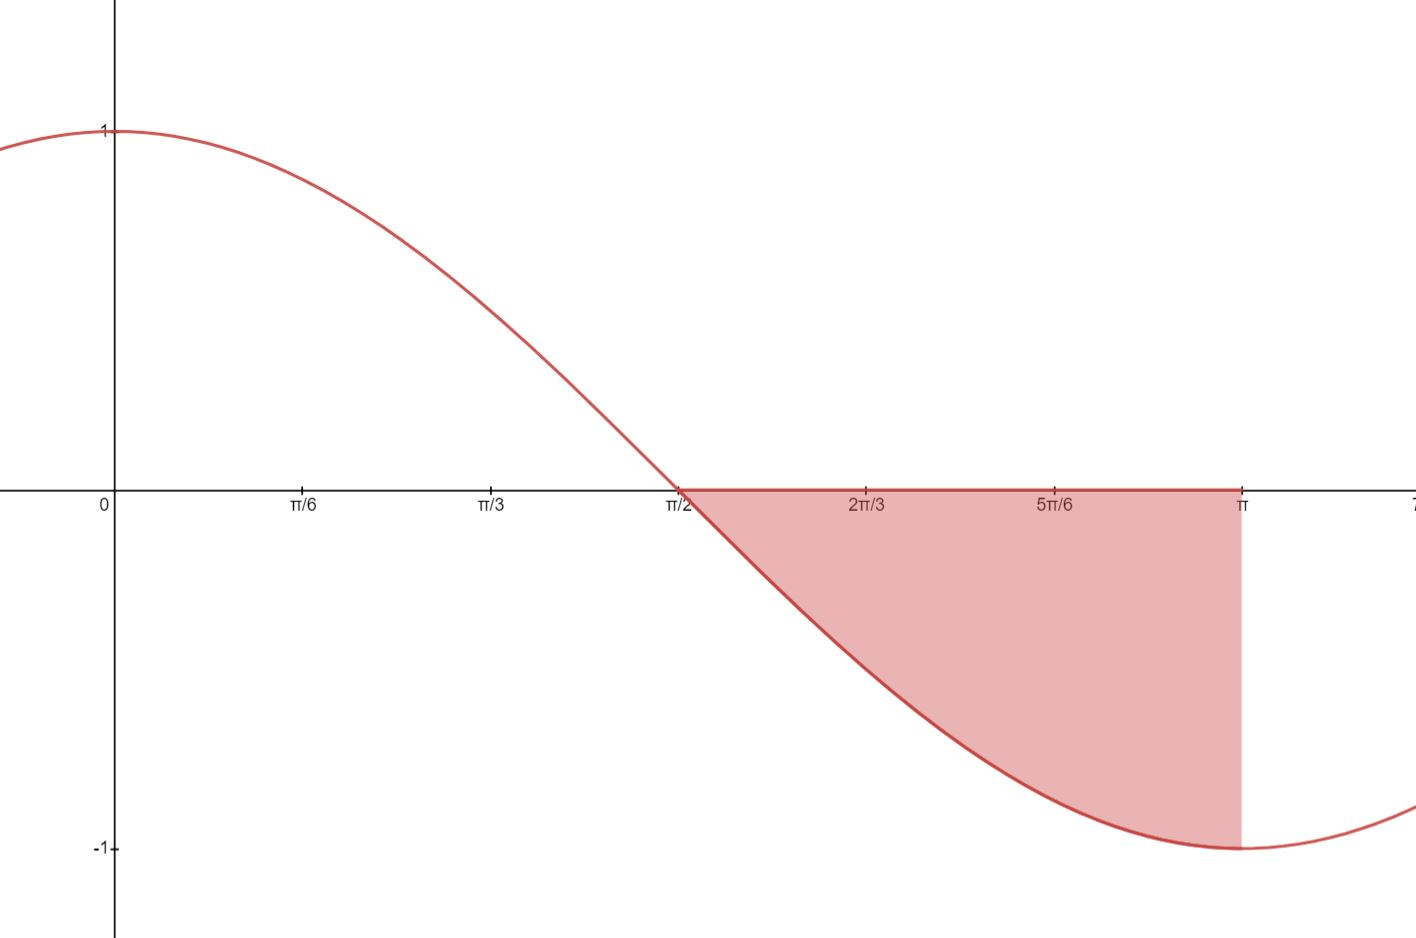
\includegraphics[scale=0.3]{fig16.JPG}}
        \caption{Area under the curve of $\cos(x)$ over $x \in [\frac{\pi}{2}, \pi]$}
        \label{fig:auccosx2}
    \end{center}
\end{figure}

\begin{center}
    * * * * *
\end{center}

When finding the area between two curves, the first step is to draw out the graphs and see which one of the two is ``on top.'' If $f(x)$ is the curve on top and $g(x)$ is the curve under, the area between the curves would be:
\[ \int_a^b f(x) - g(x) \, dx. \]
Sometimes the question may require finding the endpoints of the interval by solving for the points of intersection between the two functions.

\noindent \textbf{Examples:}
\begin{enumerate}
    \item What is area of the region between the two graphs $f(x) = x^2 + 2x + 2$ and $g(x) = 2x^2 + 3x - 4$?

          The first step is to find the endpoints of the region, which would be the points of intersection of the two functions.
          \begin{align*}
              x^2 + 2x + 2 & = 2x^2 + 3x - 4 \\
              x^2 + x - 6  & = 0             \\
              (x+3)(x-2)   & = 0             \\
              x            & = -3, \, 2
          \end{align*}

          Next, plot the two graphs to see which one is on top. (\hyperref[fig:abcx1]{Figure 17}.)

          \begin{figure}[H]
              \begin{center}
                  \frame{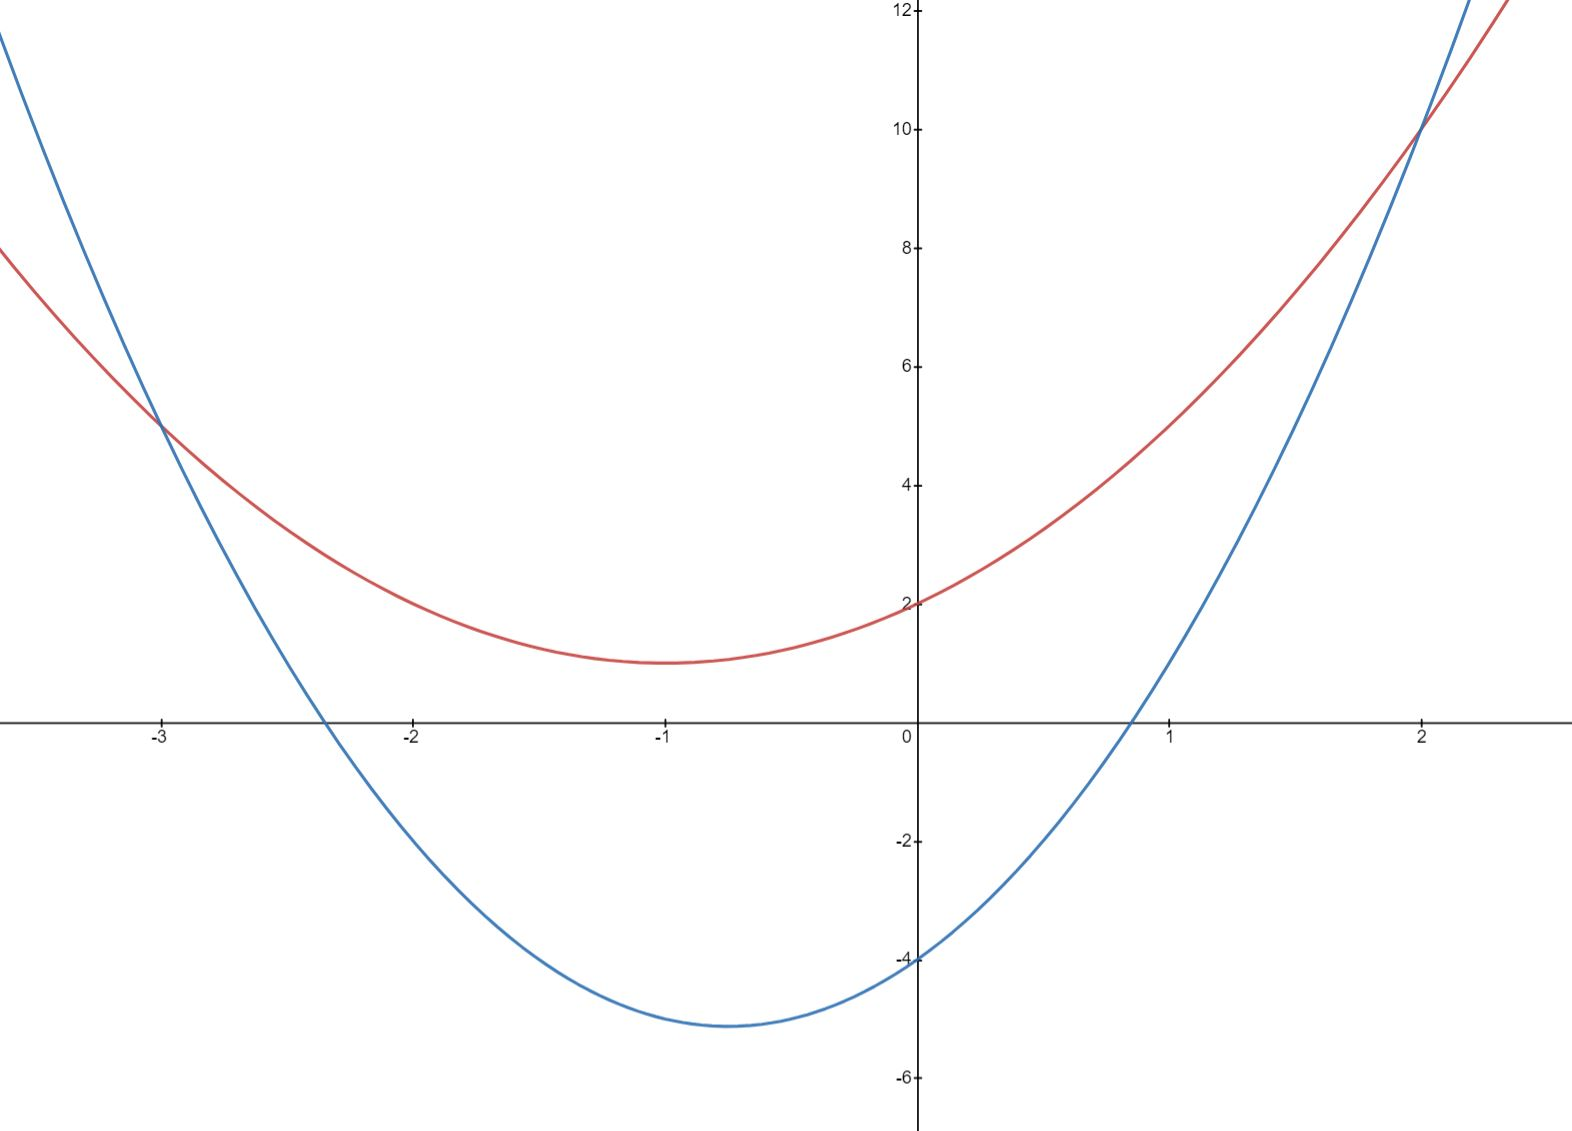
\includegraphics[scale=0.3]{fig17.JPG}}
                  \caption{$f(x)$ (top), and $g(x)$ (bottom)}
                  \label{fig:abcx1}
              \end{center}
          \end{figure}

          From the graph, we see that $f(x) \ge g(x) \, \forall \, x \in [-3, 2]$. This means we have to solve for:
          \[ \int_{-3}^2 \left( f(x) - g(x) \right) \, dx. \]
          \begin{align*}
              \int_{-3}^2 \left( f(x) - g(x) \right) \, dx & = \int_{-3}^2 \left( x^2 + 2x + 2 - 2x^2 - 3x + 4 \right) \, dx \\[6pt]
                                                           & = \int_{-3}^2 -x^2 - x + 6                                      \\[6pt]
                                                           & = \left[ -\frac{x^3}{3} -\frac{x^2}{2} + 6x \right]_{-3}^2      \\[6pt]
                                                           & = -\frac{8}{3} - 2 + 12 - 9 +\frac{9}{2} + 18                   \\[6pt]
                                                           & = \frac{125}{6}
          \end{align*}
          Therefore the area enclosed by the curves of the graphs is $\frac{125}{6}$.
          \smallskip

    \item What is the area of the region between the two graphs $f(x) = \sqrt{x+7}$ and $g(x) = 0.5(x+7)$?

          The first step is to find the endpoints of the region, which are the points of intersection of the two functions.
          \begin{align*}
              \sqrt{x+7}                         & = 0.5(x+7)    \\
              x+7                                & = 0.25(x+7)^2 \\
              0.25(x+7)^2 - (x+7)                & = 0
              (x+7) \left( 0.25(x+7) - 1 \right) & = 0
              x+7                                & = 0, \, 4     \\
              x                                  & = -7, \, -3
          \end{align*}

          Next, plot the two graphs to see which one is on top. (\hyperref[fig:abcx2]{Figure 18}.)

          \begin{figure}[H]
              \begin{center}
                  \frame{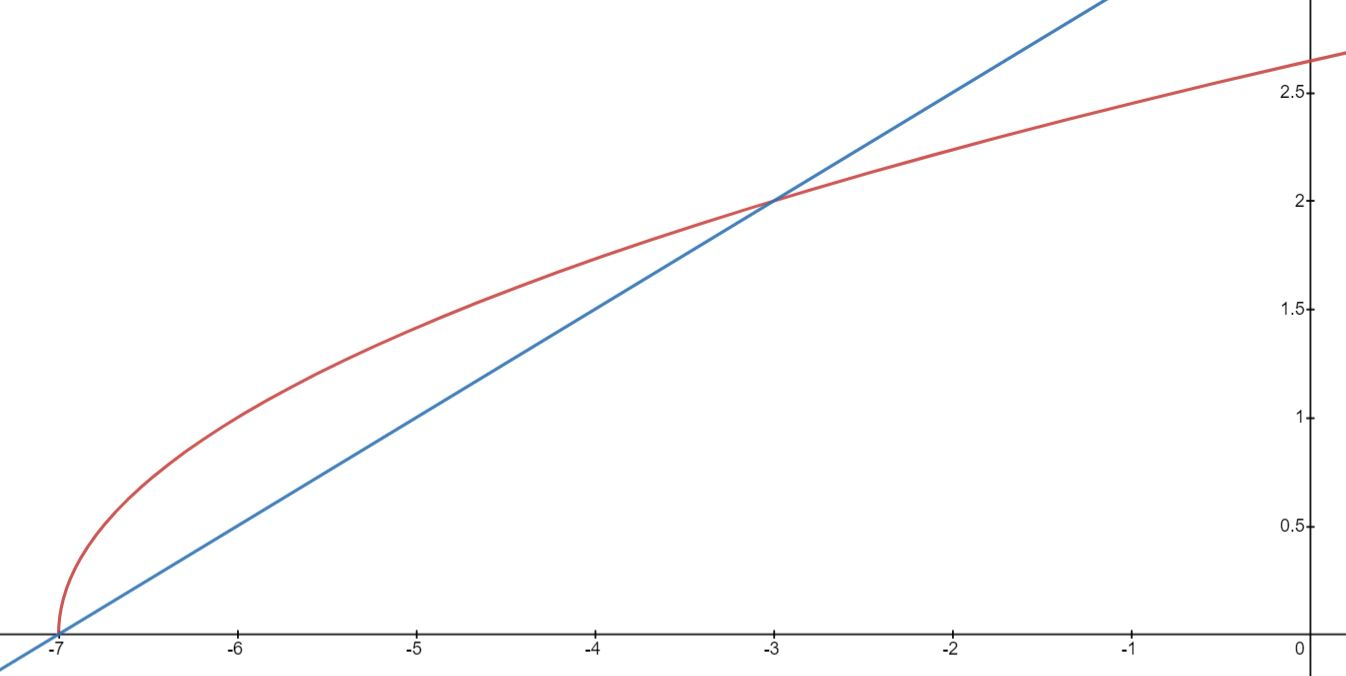
\includegraphics[scale=0.4]{fig18.JPG}}
                  \caption{$f(x)$ (top), and $g(x)$ (bottom)}
                  \label{fig:abcx2}
              \end{center}
          \end{figure}

          From the graph, we see that $f(x) \ge g(x) \, \forall \, x \in [-3, 2]$. This means we have to solve for:
          \[ \int_{-7}^{-3} \left( f(x) - g(x) \right) \, dx. \]
          \begin{align*}
              \int_{-7}^{-3} \left( f(x) - g(x) \right) \, dx & = \int_{-7}^{-3} \sqrt{x+7} - 0.5(x+7)                                      \\[6pt]
                                                              & = \left[ \frac{2(x+7)^\frac{3}{2}}{3} - \frac{(x+7)^2}{4} \right]_{-7}^{-3} \\[6pt]
                                                              & = \frac{16}{3} - 4 - 0                                                      \\[6pt]
                                                              & = \frac{4}{3}
          \end{align*}
          Therefore the area enclosed by the curves of the graphs is $\frac{4}{3}$.
\end{enumerate}

\subsubsection{Curves as Functions of y}
Finding the area between two functions of $y$ is as simple as integrating in terms of $y$. Its steps are no different than those for functions of $x$. The one difference is that the graph on the \textit{left} should be subtracted from the graph on the \textit{right}.

\noindent \textbf{Example:} Find the area between the two curves $f(y)=2y^2 + 19y + 18$ and $g(y)=7y + 18$.

\noindent First find the points of intersection for the upper and lower bound of the integral.
\begin{align*}
    2y^2 + 19y + 18 & = 7y + 18 \\
    2y^2 + 12y      & = 0       \\
    y^2 + 6y        & = 0       \\
    y(y+6)          & = 0       \\
    y = -6, \, 0
\end{align*}
Next, draw the graphs to see which one is on the left and which one is on the right. (\hyperref[fig:abcy1]{Figure 19}.)

\begin{figure}[H]
    \begin{center}
        \frame{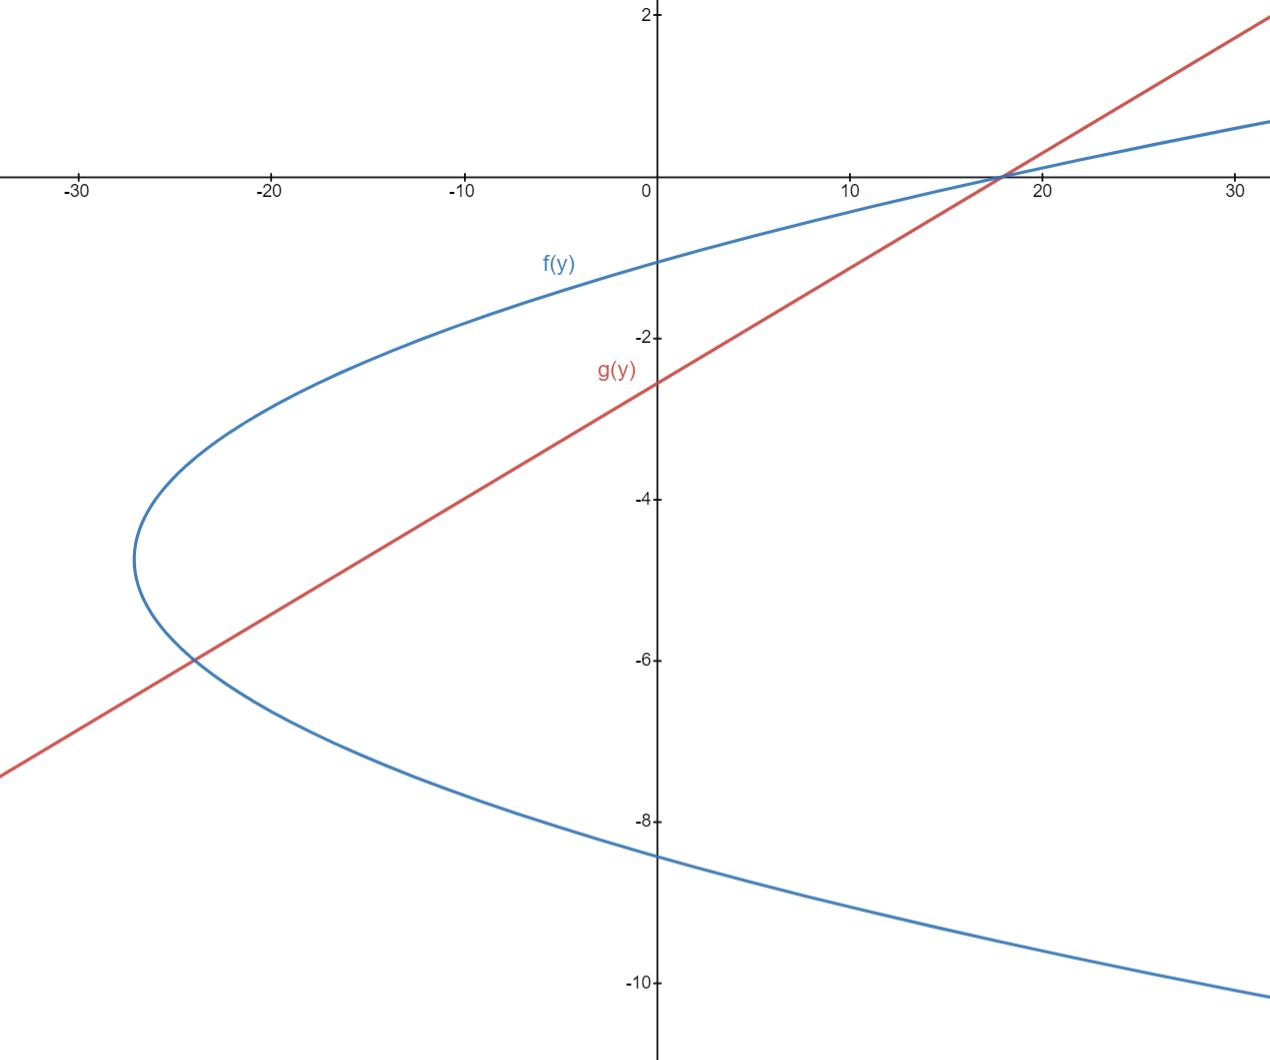
\includegraphics[scale=0.3]{fig19.JPG}}
        \caption{$f(y)$ (left), and $g(y)$ (right)}
        \label{fig:abcy1}
    \end{center}
\end{figure}

From the graph we see that $g(y)$ is on the right of $f(y)$, so the area between the curves will be:
\[ \int_{-6}^0 g(y) - f(y) \, dy. \]

\noindent Putting everything together and solving:
\begin{align*}
    \int_{-6}^0 g(y) - f(y) \, dy & = \int_{-6}^0 7y + 18 - (2y^2 + 19y + 18) \, dy \\
                                  & = \int_{-6}^0 -2y^2 - 12y \, dy                 \\
                                  & = \left[ -\frac{2y^3}{3} - 6y^2 \right]_{-6}^0  \\[6pt]
                                  & = 0 - 0 + \frac{432}{3} - 216                   \\[6pt]
                                  & = -72
\end{align*}

\subsection{Volumes with Cross Sections}
Definite integrals can also be used to find the volumes of 3D shapes. The sections below highlight a few of the more common methods in finding such volumes.

\subsubsection{Square and Rectangle Cross Sections}
% kind of hard to explain without images of the 3d shape
Given two functions, $f(x)$ and $g(x)$, where $f(x) \ge g(x) \, \forall \, x \in [a, b]$. If the graph was then extended to the $z$ axis with a given height $h$, such that all cross sections were rectangles, the volume of this figure would be:
\[ \int_a^b \left[ f(x) - g(x) \right] \cdot h \, dx. \]

If the cross sections were square then the height would be the same as the base, therefore the volume would be:
\[ \int_a^b \left[ f(x) - g(x) \right]^2 \, dx. \]
The same formula would work with functions in respect to $y$.
\bigskip

For example, let $R$ be the region enclosed by $y=\frac{x^3}{2}$, $y=4$, and the $y$ axis (\hyperref[fig:srcross]{Figure 20}). Region $R$ is the base of a solid. For each $y$-value, the cross section of the solid taken \textit{perpendicular} to the $y$-axis is a rectangle whose base lies in $R$ and whose height is $\frac{y}{2}$. \textbf{What is the definite integral needed to find the volume of the solid?}

\noindent Region $R$ is between the function and the $y$-axis, so in order to find its area with a definite integral we first need to convert the function to be in terms of $y$.
\begin{align*}
    y & = \frac{x^3}{2} \\[6pt]
    x & = \sqrt[3]{2y}
\end{align*}
We can now plug everything in to the formula to find the definite integral needed to find the volume.
\begin{align*}
    V & = \int_a^b \left[ f(y) - g(y) \right] \cdot h \, dy                \\
      & = \int_0^4 \left[ \sqrt[3]{2y} - 0 \right] \cdot \frac{y}{2} \, dy \\[6pt]
      & = \int_0^4 \sqrt[3]{2y} \cdot \frac{y}{2} \, dy
\end{align*}

\begin{figure}[H]
    \begin{center}
        \frame{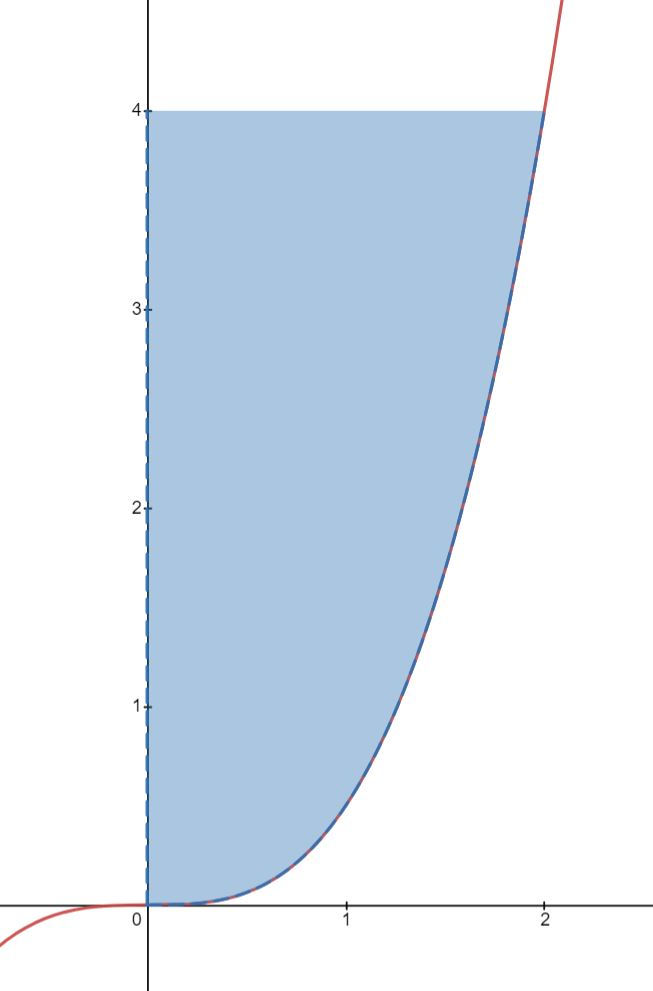
\includegraphics[scale=0.4]{fig20.JPG}}
        \caption{region $R$, shaded}
        \label{fig:srcross}
    \end{center}
\end{figure}

\subsubsection{Triangle and Semi-circle Cross Sections}
If the cross section of a shape is a triangle or semi-circle, the formula is very similar to that of a rectangle or square.
\\ For a triangle with height $h$, the formula is:
\[ \int_a^b \left[ f(x) - g(x) \right] \cdot \frac{h}{2} \, dx. \]
For a semi-circle with radius $r$, the formula is:
\[ \int_a^b \pi \cdot \left[ f(x) - g(x) \right]^2 \, dx. \]

\subsubsection{Revolving Around Axis: Disc Method}
When a shape is rotated or revolved around an axis to form a solid, its volume can be split up into an infinite amount of circles. The formula is then very similar to the area of a circle. Given $f(x) \ge g(x) \, \forall \, x \in [a, b]$, the area of the solid made by rotating the area between $f(x)$ and $g(x)$ around $g(x)$ would be:
\[ \int_a^b \pi \left( f(x) - g(x) \right)^2 \, dx. \]
For example, find the volume of the solid made by revolving the area between $f(x) = \frac{x^2}{4} + 2$ and $g(x) = 1$ over the interval $[2, 4]$ around $g(x)$ (\hyperref[fig:disc]{Figure 21}).
\begin{align*}
    V & = \int_a^b \pi \left( f(x) - g(x) \right)^2 \, dx           \\
      & = \int_2^4 \pi \left( \frac{x^2}{4} + 2 - 1 \right)^2 \, dx \\[6pt]
      & = \pi \int_2^4 \left( \frac{x^2}{4} + 1 \right)^2 \, dx     \\[6pt]
      & = \pi \int_2^4 \frac{x^4}{16} + \frac{x^2}{2} + 1 \, dx     \\[6pt]
      & = \pi \left[ \frac{x^5}{80} + \frac{x^3}{6} + x \right]_2^4 \\[6pt]
      & = \pi \left( \frac{412}{15} - \frac{56}{15} \right)         \\[6pt]
      & = \frac{356}{15} \pi
\end{align*}
Therefore the volume of the solid is $\frac{356}{15} \pi$.

\begin{figure}[H]
    \begin{center}
        \frame{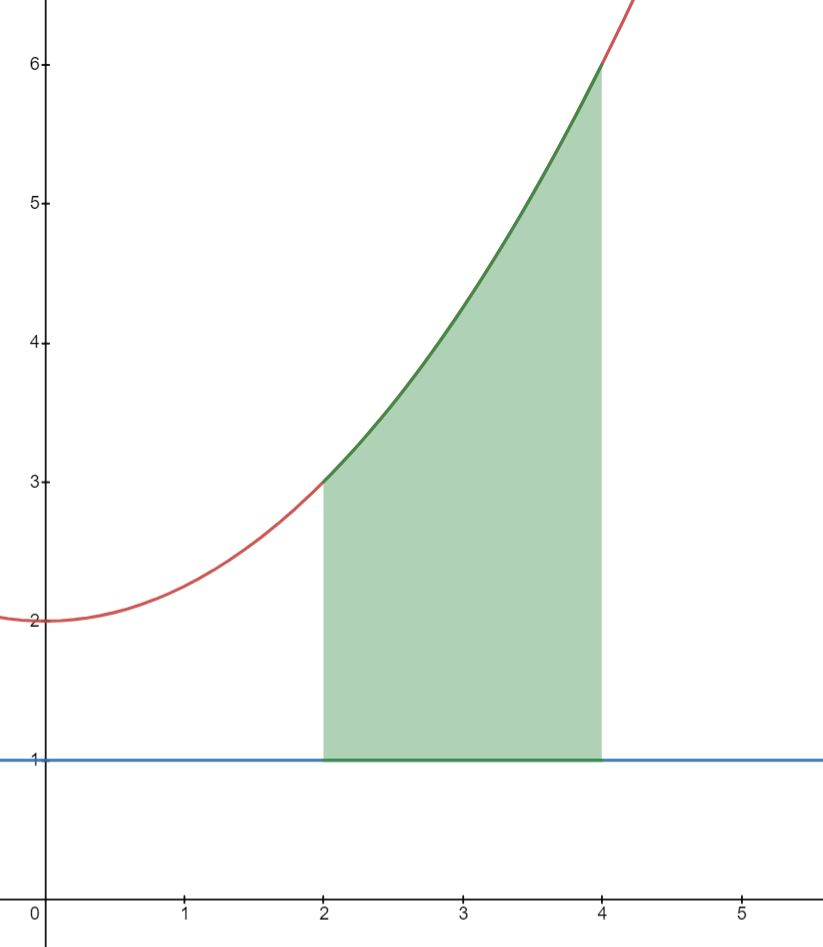
\includegraphics[scale=0.4]{fig21.JPG}}
        \caption{$f(x)$ (top), and $g(x)$ (bottom)}
        \label{fig:disc}
    \end{center}
\end{figure}

\subsubsection{Revolving Around Axis: Washer Method}
When a shape that does not have side(s) perpendicular to one of the axis is rotated around another axis to form a solid, the washer method can be used to find the volume. The idea behind this method is to find the volume of the solid formed by the top line, and subtract the volume of the solid formed by the bottom line.
\\ Given $f(x) \ge g(x) \, \forall \, x \in [a, b]$, rotating around $h(x)$, the formula is:
\[ \pi \int_a^b \underbrace{\left( f(x) - h(x) \right)^2}_{\text{solid formed by $f(x)$}} - \underbrace{\left( g(x) - h(x) \right)^2}_{\text{solid formed by $g(x)$}} \, dx.\]

\noindent \textbf{Example:}
\\ Let $R$ be the region enclosed by $f(x) = 4$, $g(x) = \frac{x^3}{2}$ and the $y$ axis (\hyperref[fig:washer]{Figure 22}). A solid is formed by rotating $R$ around $y=-1$. What is the volume of this solid? ($f(x)$ and $g(x)$ intersect at $(2, 4)$.)
\begin{align*}
    V & = \pi \int_a^b \left( f(x) - h(x) \right)^2 - \left( g(x) - h(x) \right)^2 \, dx \\
      & = \pi \int_0^2 (4+1)^2 - \left( \frac{x^3}{2} + 1 \right)^2 \, dx                \\[6pt]
      & = \pi \int_0^2 24 - \frac{x^6}{4} - x^3 \, dx                                    \\[6pt]
      & = \pi \left[ 24x - \frac{x^7}{28} - \frac{x^4}{4} \right]_0^2                    \\[6pt]
      & = \pi \left( 48 - \frac{128}{28} - 4 \right)                                     \\[6pt]
      & = \frac{276}{7} \pi
\end{align*}
Therefore the volume of the solid is $\frac{276}{7} \pi$.

\begin{figure}[H]
    \begin{center}
        \frame{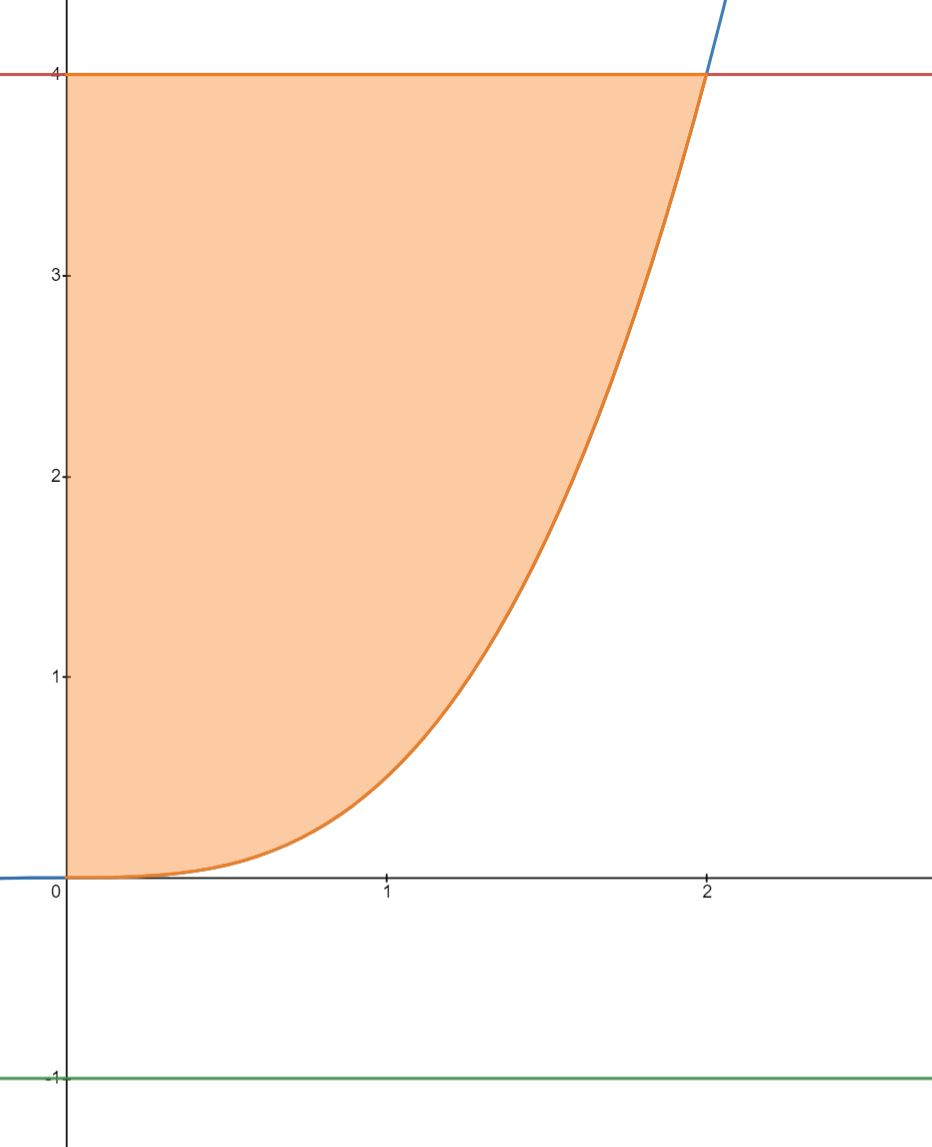
\includegraphics[scale=0.3]{fig22.JPG}}
        \caption{from top to bottom: $f(x)$, $g(x)$, $y=-1$}
        \label{fig:washer}
    \end{center}
\end{figure}

\subsection{Determining the Length of a Planar Curve}
The equation for the length of a curve of $f(x)$ in between $[a, b]$ is:
\[ \int_a^b \sqrt{1 + \left( f'(x) \right)^2} \, dx.\]

This formula comes directly from Pythagorean's Theorem. Given a function $f(x)$, split the curve up into an infinite amount of small slants, each of which will be of length $ds$ (\hyperref[fig:planarcurve]{Figure 23}).

\begin{figure}[H]
    \begin{center}
        \frame{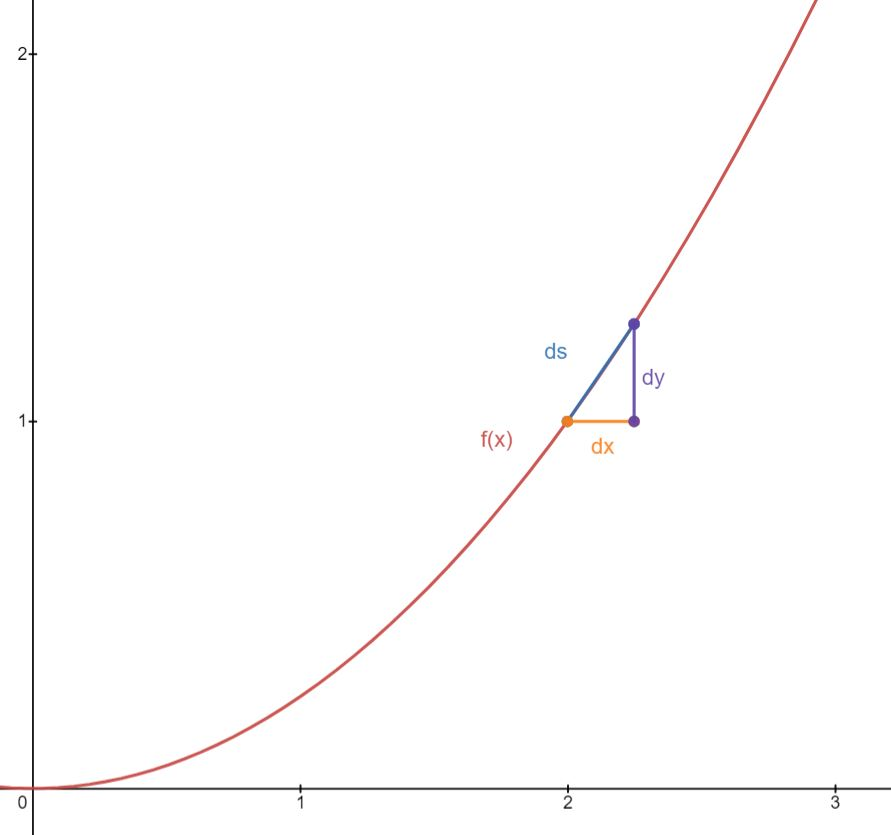
\includegraphics[scale=0.3]{fig23.JPG}}
        \caption{$f(x)$ split up into an infinite amount of $ds$'s}
        \label{fig:planarcurve}
    \end{center}
\end{figure}

\noindent The length of $f(x)$ would then be:
\[ \int ds. \]
According to Pythagorean's Theorem, we can rewrite this equation:
\begin{align*}
    ds      & = \sqrt{(dx)^2 + (dy)^2}                                      \\
    \int ds & = \int \sqrt{(dx)^2 + (dy)^2}                                 \\
            & = \int \sqrt{(dx^2) \left( 1 + \frac{(dy)^2}{(dx)^2} \right)} \\[6pt]
            & = \int \sqrt{1 + \left(\frac{dy}{dx} \right)^2} \, dx         \\[6pt]
            & = \int \sqrt{1 + \left( f'(x) \right)^2} \, dx
\end{align*}

\section{Parametric Equations, Polar Coordinates, and Vector-Valued Functions (11\% - 12\%)}
\fline

\noindent \textbf{Brief Refresher:}
\\ Parametric Equations are basically where both $x$ and $y$ are in terms of a third variable, usually $t$. For example:
\begin{align*}
    y & = 3t + 1 \\
    x & = 1 - 4t
\end{align*}

\subsection{Derivatives of Parametric and Vector-Valued Functions}
\subsubsection{First Derivative}
The key realization with taking the derivative of parametric functions is that:
\[ \frac{dy}{dx} = \frac{\frac{dy}{dt}}{\frac{dx}{dt}}. \]
For example, find the derivative of the following parametric equation:
\begin{align*}
    x & = \cos(\pi - t) \\
    y & = \tan(2t)
\end{align*}
The first step is to differentiate the two equations separately.
\begin{align*}
    \frac{dx}{dt} & = t \sin(\pi - t) \\[6pt]
    \frac{dy}{dt} & = 2 \sec(2t)
\end{align*}
We can combine these two derivatives to get the derivative of the whole function.
\begin{gather*}
    \frac{dy}{dx} = \frac{\frac{dy}{dt}}{\frac{dx}{dt}} \\[6pt]
    = \frac{2 \sec(2t)}{t \sin(\pi - t)}
\end{gather*}

\subsubsection{Higher Order Derivatives}
A higher order derivative of a parametric function is not just the derivative of the previous order derivative. It is actually taking the previous derivative with respect to $t$, then dividing by the derivative of $x$ with respect to $t$.
\\ For example, the second derivative would be:
\[ \frac{d^2 y}{dx^2} = \frac{\frac{d}{dt} \left( \frac{dy}{dx} \right)}{\frac{dx}{dt}}. \]

\subsection{Arc Lengths of Curves by Parametric Equations}
The arc length of a curve by a parametric equation is:
\[ \int_a^b \sqrt{x'(t)^2 + y'(t)^2} \, dt. \]

The arc length of parametric equations is very similar to the arc length of a normal equation. Let $dt$ by an infinitely small section of the curve, and let $dy$ be its change in $y$ and $dx$ be its change in $x$.
\begin{align*}
    \text{Length} & = \int \, dt                                                                                    \\
                  & = \int \sqrt{(dx)^2 + (dy)^2}                                                                   \\
                  & = \int \sqrt{\left( \frac{dx}{dt} \cdot dt \right)^2 + \left( \frac{dy}{dt} \cdot dt \right)^2} \\[6pt]
                  & = \int \sqrt{(dt)^2 \left( x'(t)^2 + y'(t)^2 \right)}                                           \\
                  & = \int \sqrt{x'(t)^2 + y'(t)^2} \, dt
\end{align*}

\subsection{Derivatives of Vector-Valued Functions}
The derivative of a vector valued function is just the derivative of its $x$ component and its $y$ component.
\begin{gather*}
    \vec{r}(t) = \left( x(t), \, y(t) \right) \\
    \vec{r} \, '(t) = \left( x'(t), \, y'(t) \right)
\end{gather*}
Or in unit vector notation:
\begin{gather*}
    \vec{r} = x(t) \hat{\imath} + y(t) \hat{\jmath} \\
    \vec{r} \, '(t) = x'(t) \hat{\imath} + y'(t) \hat{\jmath}
\end{gather*}
The same rule follows with higher order derivatives.

\subsection[Motion Problems With Parametric and Vector-Valued Functions]{Motion Problems With Parametric and Vector-Valued\\Functions}
The relation between position, velocity and acceleration in parametric and vector-valued functions is the same as in a normal function.
\begin{align*}
    \vec{p} \, '(t) & = \vec{v}(t) \\
    \vec{v} \, '(t) & = \vec{a}(t)
\end{align*}
Something else to remember is that the \textit{magnitude} of a vector valued function is written in the following notation:
\[ || \vec{r}(t) ||. \]
The value of the magnitude is:
\begin{align*}
    \vec{a}       & = (b, c)           \\
    || \vec{a} || & = \sqrt{b^2 + c^2}
\end{align*}

\noindent \textbf{Examples:}
\begin{enumerate}
    \item A particle moves in the $xy$ plane so that at any $t \ge 0$ its position vector is equal to $(2t^2 + 5, \, -t^3 + 4t^2)$. What is the magnitude of its acceleration vector at $t=1$?

          The first step is to find the acceleration vector. This can be done by taking the derivative of the position vector twice.
          \begin{align*}
              \vec{p}(t) & = (2t^2 + 5, \, -t^3 + 4t^2) \\
              \vec{v}(t) & = (4t, \, -3t^2 + 8t)        \\
              \vec{a}(t) & = (4, \, -6t + 8)
          \end{align*}
          Next we can plug in $t=1$ and solve for the magnitude of $\vec{a}$.
          \begin{align*}
              \vec{a}(1)       & = (4, \, 2)        \\
              || \vec{a}(1) || & = \sqrt{4^2 + 2^2} \\
                               & = 2\sqrt{5}
          \end{align*}
          Therefore the magnitude of the particle's acceleration at $t=1$ is $2\sqrt{5}$.
          \bigskip

    \item A particle moves along the curve $y=2x^2 + 2$ so that the $x$ coordinate is increasing at a constant rate of $4$ units per second. What is the magnitude of the particle's velocity vector (in units per second) when the particle is at the point $(0, \, 2)$?

          The magnitude of a particle's velocity vector is given by:
          \[ ||(\frac{dx}{dt}, \, \frac{dy}{dt})||. \]

          It is given in the question that the $x$ coordinate is changing at a constant rate of $4$ units per second. In other words, $\frac{dx}{dt} = 4$.

          We can differentiate the given function in respect to $t$ to solve for $\frac{dy}{dt}$.
          \begin{align*}
              y                & = 2x^2 + 2                \\
              \frac{d}{dt} [y] & = \frac{d}{dt} [2x^2 + 2] \\[6pt]
              \frac{dy}{dt}    & = 4x \frac{dx}{dt}        \\
                               & = 4 \cdot 0 \cdot 4       \\
                               & = 0
          \end{align*}

          Plugging everything in to solve for the magnitude:
          \begin{align*}
              ||\vec{v}(t)|| & = ||(\frac{dx}{dt}, \, \frac{dy}{dt})|| \\[6pt]
                             & = ||(4, \, 0)||                         \\
                             & = \sqrt{4^2 + 0^2}                      \\
                             & = 4
          \end{align*}
          Therefore the magnitude of the function's velocity vector is equal to $4$.
          \bigskip

    \item A particle moving in the $xy$ plane has velocity vector given by $v(t) = (2t^3, \, 3t^2)$ for time $t \ge 0$. At $t=1$, the particle's position is $(3, \, 4)$. What is the particle's position at $t=3$?

          The particle's position at $t=3$ is given by its position at $t=1$ plus its change in $x$ and $y$, respectively.
          \[ p(3) = (3 + \Delta x, \, 4 + \Delta y) \]

          We can use integrals to solve for $\Delta x$ and $\Delta y$.
          \begin{align*}
              \Delta x & = \int_1^3 2t^3 \, dt              \\
                       & = \left[ \frac{t^4}{2} \right]_1^3 \\[6pt]
                       & = \frac{81}{2} - \frac{1}{2}       \\[6pt]
                       & = 40
          \end{align*}
          And now for $\Delta y$.
          \begin{align*}
              \Delta y & = \int_1^3 3t^2 \, dt    \\
                       & = \left[ t^3 \right]_1^3 \\
                       & = 27 - 1                 \\
                       & = 26
          \end{align*}

          Plugging everything in to the equation to solve for the particle's position at $t=3$:
          \begin{align*}
              p(3) & = (3 + \Delta x, \, 4 + \Delta y) \\
                   & = (43, \, 30).
          \end{align*}
          Therefore at $t=3$, the particle is at $(43, \, 30)$.
\end{enumerate}

\subsection{Derivatives of Functions in Polar Coordinates}
When finding the derivative of functions in polar coordinates, the one important thing to remember is that:
\begin{align*}
    x & = r \cos \theta \\
    y & = r \sin \theta
\end{align*}

\noindent \textbf{For example}, given the polar curve $r=\frac{8}{\theta}$, what is the derivative of the $y$ coordinate?
\begin{align*}
    r          & = \frac{8}{\theta}                                        \\[6pt]
    y          & = r \sin \theta                                           \\
               & = \frac{8}{\theta} \cdot \sin \theta                      \\[10pt]
    y'(\theta) & = \frac{8 \theta \cos(\theta) - 8 \sin(\theta)}{\theta^2}
\end{align*}

\subsubsection{Tangent Lines in Polar Coordinates}
The slope of the tangent line in polar coordinates is equal to the change in $y$ divided by the change in $x$.
\begin{align*}
    m & = \frac{dy}{dx}                                 \\[6pt]
      & = \frac{\frac{dy}{d\theta}}{\frac{dx}{d\theta}}
\end{align*}
Another useful thing to remember is the point slope form for lines on a graph, which comes directly from the equation of the slope:
\[ y - y_1 = m(x - x_1). \]

\noindent \textbf{For example}, given the polar curve $r=\sin^2(2\theta)$, what is the equation of the tangent line of the curve at $\theta = \frac{\pi}{4}$?

\noindent The first step is to find the slope of the line, which is given by:
\[ \frac{dy}{dx}. \]
To find this we first need to find $\frac{dy}{d\theta}$ and $\frac{dx}{d\theta}$.
\begin{align*}
    y  & = r \sin \theta                                                                          \\
       & = \sin^2(2\theta) \sin \theta                                                            \\[10pt]
    y' & = 2 \cdot 2\sin(2\theta) \cos(2\theta) \sin \theta + \cos \theta \sin^2(2\theta)         \\
       & = 2 \sin(4\theta) \sin \theta + \cos \theta \sin^2(2\theta) \quad \text{(sum trig rule)}
\end{align*}
And now $\frac{dx}{d\theta}$.
\begin{align*}
    x  & = r \cos \theta                                                                  \\
       & = \sin^2(2\theta) \cos \theta                                                    \\[10pt]
    x' & = 2 \cdot 2\sin(2\theta) \cos(2\theta) \cos \theta - \sin \theta \sin^2(2\theta) \\
       & = 2\sin(4\theta) \cos \theta - \sin \theta \sin^2(2\theta)
\end{align*}
Now combining the two derivatives and evaluating at $\theta=\frac{\pi}{4}$ to find the slope of the function:
\begin{align*}
    \frac{dy}{dx} & = \frac{\frac{dy}{d\theta}}{\frac{dx}{d\theta}}                                                                              \\[6pt]
                  & = \frac{2 \sin(4\theta) \sin \theta + \cos \theta \sin^2(2\theta)}{2\sin(4\theta) \cos \theta - \sin \theta \sin^2(2\theta)} \\[6pt]
                  & = -1
\end{align*}

\noindent The next two things needed to complete the line equation are $x_1$ and $y_1$. This is just evaluating $x$ and $y$ at $\theta=\frac{\pi}{4}$.
\begin{align*}
    y_1 & = \sin^2(2\theta) \sin \theta \\
        & = \frac{\sqrt{2}}{2}          \\[10pt]
    x_1 & = \sin^2(2\theta) \cos \theta \\
        & = \frac{\sqrt{2}}{2}
\end{align*}
Plugging everything in to the line equation to get the final answer:
\begin{align*}
    y - y_1 = m(x - x_1) \\
    y - \frac{\sqrt{2}}{2} = -\left( x - \frac{\sqrt{2}}{2} \right)
\end{align*}

\subsection{Areas of Regions Bound by Polar Curves}
\subsubsection{Area Bound by a Single Polar Curve}
The area bound by a polar curve $r$ in the interval $[a, \, b]$ is equal to:
\[ \int_a^b \frac{1}{2} r^2 \, d\theta. \]

To get to this formula, imagine the area split up into an infinite amount of ``pie sections'' of radius $r$ (where the function is at that point), and of angle $d\theta$ (an infinitely small angle). The area of each one of these sections would be equal to:
\begin{align*}
    A & = \underbrace{\frac{d\theta}{2\pi}}_{\text{Fraction of} \, 2\pi} \cdot \underbrace{\pi r^2}_{\text{Area of a circle}} \\[6pt]
      & = \frac{1}{2} r^2 \, d\theta
\end{align*}
The sum of all of these sections could be found using integrals, thus the above formula.

\subsubsection{Area Bound by Two Polar Curves}
The steps in finding the area bound by polar curves is very similar to that of normal functions. First, draw out the curves to see which one is on the outside, or further away from the origin. Given two polar curves $f(\theta) \ge g(\theta) \, \forall \, \theta \in [a, \, b]$, then the area bound by the two curves is equal to:
\[ \frac{1}{2} \int_a^b \left( f(\theta) \right)^2 - \left( g(\theta) \right)^2 \, d\theta. \]

\noindent \textbf{Examples:}
\begin{enumerate}
    \item What is the area between the two polar curves $r=\pi$ and $r=\theta$ in the first two quadrants?

          First graphing the area, we see that $\pi \ge \theta$ within the first two quadrants, that is, between $0$ and $\pi$ (\hyperref[fig:abpc1]{Figure 24}).

          \begin{figure}[H]
              \begin{center}
                  \frame{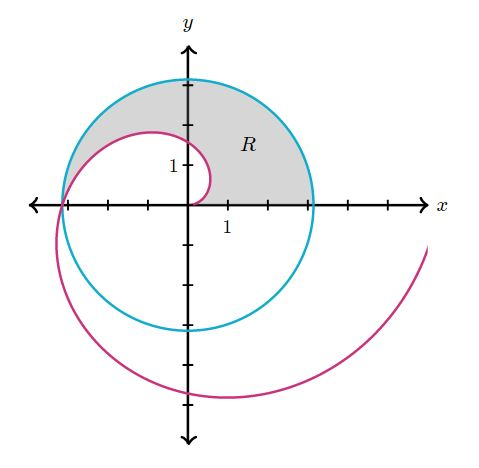
\includegraphics[scale=0.6]{fig24.JPG}}
                  \caption{Area between $r=\pi$ and $r=\theta$ in quadrant 2 (\href{https://www.khanacademy.org/math/ap-calculus-bc/bc-advanced-functions-new/bc-9-9/e/area-between-two-polar-curves?modal=1}{source})}
                  \label{fig:abpc1}
              \end{center}
          \end{figure}

          Therefore the area of this region is equal to:
          \[ \frac{1}{2} \int_0^\pi \left( \pi^2 - \theta^2 \right) \, d\theta. \]
          \bigskip

    \item What is the area between the two polar curves $r=2$ and $r=2+\cos(2\theta)$ in the fourth quadrant? The two graphs intersect at $\theta = -\frac{\pi}{4}$.

          First graphing the area, we see that it's not the case where one curve is always greater than the other (\hyperref[fig:abpc2]{Figure 25}).

          \begin{figure}[H]
              \begin{center}
                  \frame{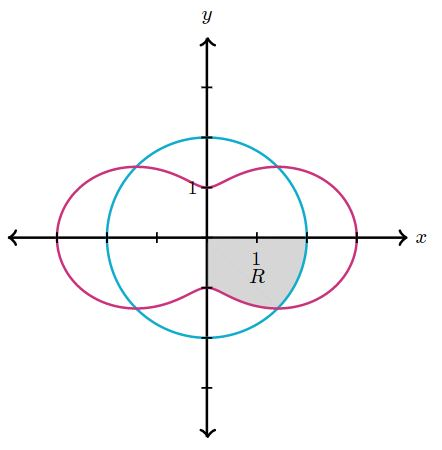
\includegraphics[scale=0.6]{fig25.JPG}}
                  \caption{Area between $r=2$ and $r=2+\cos(2\theta)$ in quadrant 4 (\href{https://www.khanacademy.org/math/ap-calculus-bc/bc-advanced-functions-new/bc-9-9/e/area-between-two-polar-curves?modal=1}{source})}
                  \label{fig:abpc2}
              \end{center}
          \end{figure}

          In order to solve for this area, we can split it up into two sections, one from $-\frac{\pi}{2}$ to $-\frac{\pi}{4}$, and the other from $-\frac{\pi}{4}$ to $0$. Notice that the two areas split at where the two graphs intersect.

          The first section (from $-\frac{\pi}{2}$ to $-\frac{\pi}{4}$) is just the area under $r=2+\cos(2\theta)$. Therefore its area is:
          \[ \frac{1}{2} \int_{-\frac{\pi}{2}}^{-\frac{\pi}{4}} \left( 2+\cos(2\theta) \right)^2 \, d\theta. \]

          The second section (from $-\frac{\pi}{4}$ to $0$) is just the area under $r=2$. Therefore its area is:
          \[ \frac{1}{2} \int_{-\frac{\pi}{4}}^0 4 \, d\theta. \]

          Combining the two areas we get that the total area bound by the two curves is equal to:
          \[ \frac{1}{2} \int_{-\frac{\pi}{2}}^{-\frac{\pi}{4}} \left( 2+\cos(2\theta) \right)^2 \, d\theta + \frac{1}{2} \int_{-\frac{\pi}{4}}^0 4 \, d\theta. \]
\end{enumerate}

\section{Infinite Sequences and Series (17\% - 18\%)}
\fline

\noindent An infinite series is the sum of an infinite number of terms in a sequence.

\subsection{Convergence and Divergence of Infinite Series}
An infinite series \textbf{converges} if $\displaystyle \lim_{n \to \infty} a_n$ approaches a value that is not $\pm \infty$. Otherwise it diverges.

\subsubsection{Partial Sums}
A partial sum is the sum of the first $n$ terms of an infinite series. It is usually represented as $S_n$. For example,
\begin{align*}
    S_1 & = \sum_{n=1}^1 a_n = a_1                           \\
    S_2 & = \sum_{n=1}^2 a_n = a_1 + a_2                     \\
    S_3 & = \sum_{n=1}^3 a_n = a_1 + a_2 + a_3               \\
    \vdots                                                   \\
    S   & = \sum_{n=1}^\infty a_n = a_1 + a_2 + a_3 + \cdots
\end{align*}

\noindent Partial sums can also be used to evaluate a term in the series.
\[ a_n = S_n - S_{n-1}. \]

\noindent For example, the $n$\textsuperscript{th} partial sum of the series $a$ is:
\[ S_n = 2 - \frac{4}{n^2}. \]
What is $a_5$?

\noindent To solve this, remember what a partial sum really is.
\[ \rlap{$\overbrace{\phantom{a_1 + a_2 + a_3 + a_4}}^{S_4}$} \underbrace{a_1 + a_2 + a_3 + a_4 + a_5}_{S_5} \]
Therefore,
\begin{align*}
    a_5 & = S_5 - S_4                                            \\
        & = 2 - \frac{4}{5^2} - \left( 2 - \frac{4}{4^2} \right) \\[6pt]
    a_5 & = \frac{9}{100}
\end{align*}

The sum of the entire sequence $a_n$ is equal to $S$. The formula to find $S$ is:
\[ S = \lim_{n \to \infty} S_n. \]
For example, given
\[ S_n = 6n + \frac{1}{n^3} \]
what is $S$?
\begin{align*}
    S & = \lim_{n \to \infty} S_n                \\
      & = \lim_{n \to \infty} 6n + \frac{1}{n^3} \\[6pt]
      & = \infty
\end{align*}
Therefore $S$ is equal to infinity and it diverges.

\subsection{Types of Series}
% Arithmetic, Geometric, Harmonic, P-series
% When do each converge and diverge
\subsubsection{Arithmetic Series}
Arithmetic series are where each term is derived from the previous term by adding or subtracting a constant. (E.g. $1, 3, 5, 7, 9, \cdots$)
\[ \sum_{n=1}^\infty (a_1 + d(n-1)) \]
\textbf{Convergent}: never
\\ \textbf{Divergent}: always

\subsubsection{Geometric Series}
Geometric series are where each term is derived from the previous term by multiplying or dividing a constant. (E.g. $1, 2, 4, 8, 16, \cdots$)
\[ \sum_{n=1}^\infty a_1r^{n-1} \]
\textbf{Convergent}: $|r| < 1$ with $S = \frac{a_1}{1-r}$ (sum of infinite geometric series)
\\ \textbf{Divergent}: $|r| \ge 1$

\subsubsection{P-Series}
A p-series is a special type of geometric series. Their general form can be written as ($p$ is constant):
\[ \sum_{n=1}^\infty \frac{1}{n^p} \]
\textbf{Convergent}: $p > 1$
\\ \textbf{Divergent}: $0 < p \le 1$

\subsubsection{Harmonic Series}
The harmonic series is a specific p-series where $p=1$.
\[ \sum_{n=1}^\infty \frac{1}{n} \]
\textbf{Convergent}: never
\\ \textbf{Divergent}: always

\subsection{Convergence and Divergence Tests}
\subsubsection{Divergence Test}
If $\displaystyle \lim_{n \to \infty} a_n \ne 0$ then $\displaystyle \sum_{n=1}^\infty a_n$ diverges.

\subsubsection{Integral Test for Convergence}
Given $f(x)$ is a \underline{positive and decreasing} function over the interval $[k, \, \infty)$, such that $f(n) = a_n$, then:

\noindent If $\displaystyle \int_k^\infty f(x) \, dx$ converges so does $\displaystyle \sum_{n=k}^\infty a_n$.

\noindent If $\displaystyle \int_k^\infty f(x) \, dx$ diverges so does $\displaystyle \sum_{n=k}^\infty a_n$.

\subsubsection{Comparisson Test}
Given two series $\displaystyle \sum a_n$ and $\displaystyle \sum b_n$ such that $a_n, \, b_n \ge 0$ for all $n$ and $a_n \ge b_n$ for all $n$, then:

\noindent If $\displaystyle \sum a_n$ converges so does $\displaystyle \sum b_n$.

\noindent If $\displaystyle \sum b_n$ diverges so does $\displaystyle \sum a_n$.

\noindent (If the lower one diverges the upper one can't converge, and if the upper one converges the lower one can't diverge.)

\subsubsection{Alternating Series Test}
Given a series $\displaystyle \sum a_n$ and either $a_n = (-1)^n b_n$ or $a_n = (-1)^{n+1} b_n$ where $b_n \ge 0$ for all $n$. Then if:
\[ \lim_{n \to \infty} b_n = 0 \quad \text{and} \quad \{b_n\} \, \text{is a decreasing sequence} \]
then $\displaystyle \sum a_n$ converges.

\subsubsection{Ratio Test}
\noindent Given a series $\displaystyle \sum a_n$, let
\[ L = \lim_{n \to \infty} \left| \frac{a_{n+1}}{a_n} \right|. \]

\noindent If $L < 1$ the series converges absolutely.
\\ If $L > 1$ the series diverges.
\\ If $L = 1$ the test is inconclusive.

\subsubsection{Absolute vs Conditional Convergence}
\noindent A series $\displaystyle \sum a_n$ is \textbf{absolutely convergent} if $\displaystyle \sum |a_n|$ is convergent.

\noindent If $\displaystyle \sum a_n$ is convergent and $\displaystyle \sum |a_n|$ is divergent than it is \textbf{conditionally convergent}.

\subsection{Power Series}
A power series is any series that can be written in the form of:
\[ \sum_{n=0}^\infty a_n (x-c)^n. \]
where $a_n$ and $c$ are numbers. The power series can be written as a function of $x$.

\noindent An example of a power series is:
\[ \sum_{n=1}^\infty \frac{(-1)^n n}{4^n} (x+3)^n. \]

\subsubsection{Radius and Interval of Convergence}
\noindent If a power series converges such that
\[ |x-c| < R \]
then $R$ is called the \textbf{radius of convergence}. The \textbf{interval of convergence} is just the radius of convergence rewritten as an interval.
\[ c - R < x < c + R \]

To determine that radius or interval of convergence for a power series, simply use any one of the convergence tests. The ratio test is usually very effective.

\noindent \textbf{Examples}:
\begin{enumerate}
    \item Find the radius and interval of convergence for the following power series:
          \[ \sum_{n=1}^\infty \frac{(-1)^n n}{4^n} (x+3)^n. \]

          The ratio test is one way to solve this. The series will converge if:
          \[ \lim_{n \to \infty} \left| \frac{a_{n+1}}{a_n} \right| < 1. \]
          Plugging in the given series:
          \begin{align*}
               & \lim_{n \to \infty} \left| \frac{(-1)^{n+1}(n+1)(x+3)^{n+1}}{4^{n+1}} \cdot \frac{4^n}{(-1)^n (n)(n+3^n)} \right| < 1 \\[6pt]
               & \lim_{n \to \infty} \left| \frac{-(n+1)(x+3)}{4n} \right| < 1                                                         \\[6pt]
          \end{align*}
          Keep in mind that $x$ is not actually part of the limit, so it can be written on the outside of the limit.
          \begin{align*}
              |x+3| \cdot \lim_{n \to \infty} \frac{n+1}{4n} & < 1 \\[6pt]
              \frac{1}{4} |x+3|                              & < 1 \\[6pt]
              |x+3|                                          & < 4
          \end{align*}
          Therefore the radius of convergence for the power series is $|x+3| < 4$. Now to find the interval of convergence:
          \begin{gather*}
              |x+3| < 4 \\
              -4 < x+3 < 4 \\
              -7 < x < 1.
          \end{gather*}
          The final step is to see if either of the endpoints will cause the series to converge.

          First testing out $x=1$:
          \begin{gather*}
              \sum_{n=1}^\infty \frac{(-1)^n n}{4^n} (1+3)^n \\[6pt]
              \sum_{n=1}^\infty (-1)^n n
          \end{gather*}
          By the alternating series test this series diverges.

          Next testing out $x=-7$:
          \begin{align*}
              \sum_{n=1}^\infty \frac{(-1)^n n}{4^n} (-7+3)^n \\[6pt]
              \sum_{n=1}^\infty (-1)^{n+1} n
          \end{align*}
          By the alternating series test this series also diverges.

          It can thus be concluded that the interval of convergence for the original series is $-7 < x < 1$.
          \bigskip

    \item Find the radius and interval of convergence for the following power series:
          \[ \sum_{n=1}^\infty \frac{4(x-5)^n}{n^2 (-4)^n}. \]

          The ratio test can be used to solve this. The series converges if:
          \[ \lim_{n \to \infty} \left| \frac{a_{n+1}}{a_n} \right| < 1. \]
          Plugging in the given series and solving:
          \begin{gather*}
              \lim_{n \to \infty} \left| \frac{4(x-5)^{n+1}}{(n+1)^2 (-4)^{n+1}} \cdot \frac{n^2 (-4)^n}{4(x-5)^n} \right| < 1 \\[6pt]
              \lim_{n \to \infty} \left( \frac{n^2}{4(n+1)^2} \right) \cdot |x-5| < 1 \\[6pt]
              \frac{|x-5|}{4} < 1 \\[6pt]
              |x-5| < 4 \\
              1 < x < 9
          \end{gather*}
          Now to check if either if the series converges at either of the endpoints. First testing out $x=9$:
          \begin{gather*}
              \sum_{n=1}^\infty \frac{4(9-5)^n}{n^2 (-4)^n} \\[6pt]
              \sum_{n=1}^\infty \frac{4}{n^2} \cdot (-1)^{n+1}
          \end{gather*}
          By the alternating series test this series converges.

          Next testing $x=1$:
          \begin{gather*}
              \sum_{n=1}^\infty \frac{4(1-5)^n}{n^2 (-4)^n} \\[6pt]
              \sum_{n=1}^\infty \frac{4}{n^2} \cdot (-1)^{n}
          \end{gather*}
          By the alternating series test this series also converges.

          Therefore the interval of convergence for the original series is $1 \le x \le 9$.
\end{enumerate}

\subsection{Taylor and Maclaurin Series}
\noindent The \textbf{Taylor Series} centered at $c$ of $f(x)$:
\begin{align*}
    f(x) & = \sum_{n=0}^\infty \frac{f^{(n)}(c)}{n!} (x-c)^n                                   \\
         & = f(c) + f'(c)(x-c) + \frac{f''(c)(x-c)^2}{2!} + \frac{f'''(c)(x-c)^3}{3!} + \cdots
\end{align*}
The $n$\textsuperscript{th} degree Taylor polynomial of $f(x)$ is:
\[ T_n(x) = \sum{i=0}^n \frac{f^{(i)}(c)}{i!} (x-c)^i. \]
The \textbf{Maclaurin Series} is just the Taylor Series centered at $0$:
\begin{align*}
    f(x) & = \sum_{n=0}^\infty \frac{f^{(n)}(0)}{n!} x^n                           \\
         & = f(0) + f'(0)x + \frac{f''(0)x^2}{2!} + \frac{f'''(0)x^3}{3!} + \cdots
\end{align*}

\subsubsection{Lagrange Error Bound}
\noindent The error of a Taylor polynomial is equal to:
\[ R_n = f(x) - T_n(x). \]

\noindent The Lagrange Error Bound for $R_n(x)$, the error of approximating $f(x)$ with the $n$\textsuperscript{th} Taylor polynomial of $f$ about $c$ is:
\[ |R_n(x)| \le \left| \frac{M}{(n+1)!} (x-c)^{n+1} \right|. \]
Where $M$ is the maximum value of $f^{(n+1)}(z)$ for any value $z$ between $x$ and $c$.

\noindent \textbf{Examples:}
\begin{enumerate}
    \item Estimating $\sin(-0.1)$ using a Maclaurin polynomial, what is the least degree of polynomial that assures an error smaller than $0.001$?

          The absolute value for the $(n+1)$\textsuperscript{th} derivative of $\sin(x)$ is never more than $1$. Its derivatives go through the cycle:
          \begin{gather*}
              \sin(x) \\
              \cos(x) \\
              -\sin(x) \\
              -\cos(x)
          \end{gather*}

          We can now plug in what we know into the Lagrange Error Bound. Note that $c=0$ because this is a Maclaurin Series.
          \begin{align*}
              |R_n(-0.1)| & \le \left| \frac{1}{(n+1)!} (-0.1)^{n+1} \right| \\
                          & = \frac{(-0.1)^{n+1}}{(n+1)!}
          \end{align*}
          The inequality to satisfy is:
          \[ \frac{(-0.1)^{n+1}}{(n+1)!} < 0.001 \]
          Through trial and error we find that the smallest possible $n$ is $2$.

          Therefore the least degree polynomial that assures an error smaller than $0.001$ is $n=2$.
          \bigskip

    \item Estimating $\ln(1.7)$ using a Taylor polynomial about $x=2$, what is the least degree of the polynomial that assures an error smaller than $0.001$?
          \\ (The $n$\textsuperscript{th} derivative of $\ln(x)$ for all $n \ge 1$ is:)
          \[ (-1)^{n+1} \frac{(n-1)!}{x^n}. \]

          The maximum value for the $(n+1)$\textsuperscript{th} derivative of $\ln(x)$ is:
          \[ \frac{n!}{x^{n+1}}. \]
          Where $x$ is between $1.7$ and $2$. It can be proven that $x=1.7$ would yield a greater result.

          Plugging in everything into the Lagrange Error Bound:
          \begin{align*}
              |R_n(1.7) & \le \left| \frac{n!}{1.7^{n+1}} \cdot \frac{1}{(n+1)!} \cdot (1.7-2)^{n+1} \right| \\[6pt]
                        & = \frac{(0.3)^{n+1}}{(1.7)^n (n+1)}
          \end{align*}
          The inequality to satisfy is:
          \[ \frac{(0.3)^{n+1}}{(1.7)^n (n+1)} < 0.001 \]
          Through trial and error we find that the smallest possible $n$ is $3$.

          Therefore the least degree polynomial that assures an error less than $0.001$ is $n=3$.
\end{enumerate}

\subsubsection{Important Maclaurin Series}
\noindent Some important Maclaurin Series that may be useful in solving problems:
\begin{align*}
     & e^x = \sum_{n=0}^\infty \frac{x^n}{n!} = 1 + x + \frac{x^2}{2!} + \frac{x^3}{3!} + \cdots                                   \\[6pt]
     & \cos(x) = \sum_{n=0}^\infty \frac{(-1)^n x^{2n}}{(2n)!} = 1 - \frac{x^2}{2!} + \frac{x^4}{4!} - \frac{x^6}{6!} + \cdots     \\[6pt]
     & \sin(x) = \sum_{n=0}^\infty \frac{(-1)^n x^{2n+1}}{(2n+1)!} = x - \frac{x^3}{3!} + \frac{x^5}{5!} - \frac{x^7}{7!} + \cdots
\end{align*}

\subsubsection{Function as a Geometric Sequence}
\noindent Note that the sum of an infinite geometric sequence is:
\[ \frac{a}{1-r} \]
Where $a$ is the first term and $r$ is the common ratio.

\noindent So if a function follows roughly the same structure it can be rewritten as a geometric sequence. For example,
\[ f(x) = \frac{1}{3+x^2} \]
resembles the sum of a geometric sequence. We can rearrange it to have it closer resemble the sum.
\begin{align*}
    f(x) & = \frac{1}{3+x^2}                       \\[6pt]
         & = \frac{\frac{1}{3}}{1 + \frac{x^2}{3}}
\end{align*}
Therefore the first term is $\frac{1}{3}$ and the common ratio is $-\frac{x^2}{3}$. The series can thus be written as:
\[ \frac{1}{3} - \frac{x^2}{9} + \frac{x^4}{27} + \cdots. \]

\subsection{Error Bounds of Convergent Infinite Series}
\subsubsection{Alternating Series Error Bound}
An alternating series can be approximated by finding the sum of its first $k$ elements. The sum of the remaining terms will be the \textbf{remainder}.
\begin{gather*}
    \sum_{n=1}^\infty a_n = \sum_{n=1}^k a_n + \sum_{n=k+1}^\infty a_n \\[10pt]
    S = \underbrace{S_k}_{\text{approximation}} + \underbrace{\sum_{n=k+1}^\infty a_n}_{\text{remainder}}
\end{gather*}
The remainder for the sum of the first $k$ elements is usually written as $R_k$.
\begin{gather*}
    R_k = a_{k+1} + a_{k+2} + a_{k+3} + \cdots \\
    S = S_k + R_k
\end{gather*}
Because $a$ is an alternating series, $R_k$ can be either positive or negative. The sign of $R_k$ is equal to the sign of $a_{k+1} + a_{k+2}$. If $R_k$ is positive, then the approximation is an \underline{underestimate} of $S$. Otherwise the approximation is an \underline{overestimate} of $S$.

\noindent Another relation between the remainder and the series is:
\[ |R_k| \le |a_{k+1}| \le |\text{error}|. \]
(`error' is explained in the example below)

\noindent \textbf{Example}:
\[ \sum_{n=1}^\infty \frac{(-1)^{n+1}}{n^4} \]
Using the alternate series test, what is the least number of terms necessary to approximate the series to within $\pm 0.0001$ of the actual value?
\begin{align*}
    |a_{k+1}|                                 & \le |\text{error}| \\[6pt]
    \left| \frac{(-1^{k+2})}{(k+1)^4} \right| & \le |\pm 0.0001|   \\[6pt]
    \frac{1}{(k+1)^4}                         & \le 0.0001         \\[6pt]
    10000                                     & \le (k+1)^4        \\
    k+1                                       & \ge 10             \\
    k                                         & \ge 9
\end{align*}
Therefore the least number of terms necessary to approximate the series to within $\pm 0.0001$ of the actual value is $9$.
\end{document}
